\documentclass[twoside]{article}

%\usepackage{aistats2022}
% If your paper is accepted, change the options for the package
% aistats2022 as follows:
%

\usepackage{aistats2022}
\usepackage{amsthm}
\usepackage{amsfonts}
\usepackage{amsmath}
\usepackage{amssymb,bbm}
\usepackage{algorithm,algorithmic}
\usepackage{natbib}
\usepackage{graphicx}
\usepackage{bm}
\usepackage{dsfont}
%
% This option will print headings for the title of your paper and
% headings for the authors names, plus a copyright note at the end of
% the first column of the first page.

% If you set papersize explicitly, activate the following three lines:
\special{papersize = 8.5in, 11in}
\setlength{\pdfpageheight}{11in}
\setlength{\pdfpagewidth}{8.5in}
% If you use natbib package, activate the following three lines:
%\usepackage[round]{natbib}
%\renewcommand{\bibname}{References}
%\renewcommand{\bibsection}{\subsubsection*{\bibname}}

% If you use BibTeX in apalike style, activate the following line:
%\bibliographystyle{apalike}
\theoremstyle{plain}
\newtheorem{thm}{Theorem}
\newtheorem*{thm*}{Theorem}
\newtheorem{lem}[thm]{Lemma}
\newtheorem{prop}[thm]{Proposition}
\newtheorem{cor}[thm]{Corollary}
\newtheorem{conj}[thm]{Conjecture}

\newcommand{\calC} {\mathcal{C}}
\newcommand{\bfP} {\mathbf{P}}
\newcommand{\kl}{\mathbf {KL}}
\newcommand{\kll}{\mathcal {KL}}
\newcommand{\OTmp}[1]{\hat{\mathbf{P}}_{#1}}
\newcommand{\prox}{\operatorname{prox}}
\newcommand{\proj}{\operatorname{Proj}}
\newcommand{\diag}{\operatorname{diag}}
\newcommand{\argmin}{\operatorname{argmin}}
%\newcommandT{\mathsf T}
%\newcommandT{T}
\newcommand{\R}{\mathbb{R}}
\newcommand{\one}{\mathds{1}}
\newcommand{\mat}[1]{\mathbf{#1}}
%\renewcommand{\vec}[1]{\mathbf{#1}}
\renewcommand{\vec}[1]{\bm{#1}}

\usepackage{xcolor}    
\newcommand{\changeHK}[1]{\textcolor{red}{#1}}
\newcommand{\changeXS}[1]{\textcolor{blue}{#1}}
\newcommand{\note}[1]{\textcolor{magenta}{#1}}

\begin{document}

% If your paper is accepted and the title of your paper is very long,
% the style will print as headings an error message. Use the following
% command to supply a shorter title of your paper so that it can be
% used as headings.
%
%\runningtitle{I use this title instead because the last one was very long}

% If your paper is accepted and the number of authors is large, the
% style will print as headings an error message. Use the following
% command to supply a shorter version of the authors names so that
% they can be used as headings (for example, use only the surnames)
%
%\runningauthor{Surname 1, Surname 2, Surname 3, ...., Surname n}

\twocolumn[

\aistatstitle{Safe Screening for $\ell_2$-norm Penalized Unbalanced Optimal Transport}

\aistatsauthor{ Xun Su \And Author 2 \And  Author 3 }

\aistatsaddress{Waseda University \And  Institution 2 \And Institution 3 } ]

%\begin{abstract}
This paper builds the dynamic screening framework on the Unbalanced Optimal Transport (UOT) problem. Recently, researchers have connected the UOT problem with Lasso problem, which encourage us to combine the widely used technique in Lasso problem, Dynamic Screening, with the UOT problem. We demonstrate the effectiveness of the screening method for UOT problem and propose improvements based on the unique structure of the UOT problem. We constructed several experiments and prove the effectiveness of our method. 

\end{abstract}


%\section{Introduction}
Optimal Transport (OT) has a long history in mathematics and prevailed recently due to its important role in measuring the distance between histograms in the Machine Learning community. It outperforms the traditional method in many fields like domain adaptation \citep{7586038}, generative model \citep{arjovsky2017wasserstein}, graph machine learning \citep{NEURIPS2019_fdd5b16f} and natural language processing. \citep{084adf2f555549c493e0331a00e4ecad} Its popularity is attributed to the introduction of the Sinkhorn algorithm to the entropic optimal transport problem, \citep{NIPS2013_af21d0c9} which improved the computational speed of OT problem from $\Theta (n^3)$ of Simplex method to $\Theta (n^2)$. However, Optimal transport problem can only deal with balanced samples, which limits its application in various data structures. Unbalanced Optimal Transport (UOT) problem has been promoted to deal with the drawback on unbalanced samples. Traditional Sinkhorn method can deal with an entropic UOT problem as well, but suffered from the slow convergence rate of the large penalty part and a non sparse solution, It can also be solved with other methods like Majorization-Minimization and FISTA method according to the choice of the penalty function in the primal problem and the Lagrange method for dual problem\citep{NEURIPS2021_c3c617a9}. UOT problem has a similar structure with many other famous problems like Non-negative Matrix Factorization and Lasso problem, which encourage the researchers to use the abundant results in these field to improve it.

Screening is a famous method in Lasso problem field, the $L_1$ penalize function causes a sparse solution for problem, which constrains many elements of solution equal to zero. The large scale optimization problem suffers from the computational process for manipulating on these zeros elements. \citep{ghaoui2010safe} invented the safe screening, which could theoretically judge whether the elements in solution equal to zero. It freezed the identified elements with linear complexity computation and save optimization time. Many new methods have been promoted to revise the method, \citep{JMLR:v18:16-577} invented the dynamic screening to dynamically screening out zeros elements, and there are many paper tries to improve it.  

Fortunately, the OT function in UOT problem has the same effectiveness as $L_1$ in lasso and cause a sparse solution. We believe that this method could be applied on UOT problem and have better performance than ordinal Lasso problem for its special structure.

\textbf{Contribution}: 
\begin{itemize}
\item We systematically combine the framework of Screening method on UOT problem, and we give a correct projection method for UOT screening, which is better than the Lasso one. 
\item We also imporve the constraints construction method for the specific sparse structure of UOT problems and benefits from it.
\end{itemize}




%\section{BACKGROUND}
\subsection{Optimal Transport and Unbalanced Optimal Transport}
Given two histograms $\ma\in \R^{m}, \mb \in \R^{n},$ For a cost matrix $\C \in \mathbbm{R_{+}}^{m \times n}$, mordern Optimal transport problem is trying to get a corresponding transport matrix $\T \in \R_{+}^{m \times n}$ that minimize the whole transport cost, which could be formulated as:
\begin{equation}
\begin{split}
&\operatorname{OT}(\ma,\mb) := \min_{ \T \in \R_{+}^{n \times n}} \langle \C, \T \rangle \\
& \mathbf{T} \one_n= \ma, \mathbf{T}^{T}\one_m = \mb
\end{split}
\end{equation}

We can write it into a vector type, set $\vc,\vt \in \mathbbm{R}^{mn}$:
\begin{equation}
\begin{split}
&\operatorname{OT}(\ma,\mb) := \min_{t \in \R_{+}^{n^2}} c^{\tranT}\vt \\
& \mathbf{N}\vt = \alpha, \mathbf{M}\vt = \beta
\end{split}
\end{equation}

$\mathbf{N} \in \R^{m \times mn}, \mathbf{N} \in \R^{n \times mn}$ are two matrix consisted with 0 and 1, listed in Appendix.A. When the $\|\ma\|_2 = \|\mb\|_2$, it is the OT problem. When $\|\ma\|_2 \neq \|\mb\|_2$, the solution $\hat{\vt}$ is not exist. We define $\y = [\ma, \mb]^{\tranT}$, the UOT problem uses a penalty function for the historgrams: 
\begin{equation}
\label{eq:uot}
\operatorname{UOT}(\ma,\mb) := \min_{\vt \in \R_{+}^{mn}} \vc^{\tranT}t + D_h(\X\vt,\y)
\end{equation}
$D_h$ is the Bregman divergence derived from the norm $h$, $\X = [\mathbf{M}^{\tranT} \mathbf{N}^{\tranT}]^{\tranT}$. 

\subsection{Relationship with Lasso}
The lasso-like problem has a general formula:
$$
\begin{aligned}
f(\vt) = g(\vt) + D_h(\X \vt,\y), t\in \mathbbm{R}^{mn}
\end{aligned}
$$
When $g(\vt) = \lambda \|\vt\|_1$ and $D_h(\X \vt,\y) = \|\X \vt-\y\|_2^2$, this is the $L_2$ regression Lasso problem. It is important to note that $\X$ in UOT is a bit different from the $\X$ in the Lasso problem, the former $\X$ has a specific structure and has only two non-zero elements and is equal to 1, which is quite different to the irregular and dense $\X$ in Lasso problem.


\subsection{Dynamic Screening Framework}

We follow \citep{NEURIPS2021_7b5b23f4}'s framework to introduce the whole dynamic screening technique for the Lasso-like problem:
\begin{equation}
\label{eq:lassolike}
f(\vt) = g(\vt) + d(\X \vt)
\end{equation}

By Frenchel-Rockafellar Duality, we get the dual problem
\begin{thm}
 (Frenchel-Rockafellar Duality) If $d$ and $g$ are proper convex functions on $\mathbbm{R}^{m+n}$ and $\mathbbm{R}^{mn}$. Then we have the following:
 $$
\begin{aligned}
\min_\vt g(\vt) + d(\X\vt) = \max_{\theta} -d^*(-\theta)-g^*(\X^{\tranT}\theta)
\end{aligned}
$$
\end{thm}

Because the primal function $d$ is always convex, the dual function $d^*$ is concave. Assuming $d^*$ is an L-strongly concave problem. we can design an area for any feasible $\tilde{\theta}$ by the strongly concave property:

\begin{thm}\label{circle}
(L-strongly concave) Considering problem \ref{eq:lassolike}, if function $d$ and $g$ are both convex, for $\forall \tilde{\theta} \in{R^{m+n}}$ and satisfied the constraints on the dual problem, we have the following area constructed by its L-strongly concave property:  
$$
\begin{aligned}
\mathcal{R}^{C}:=\theta \in \{\frac{L}{2}\|\theta-\tilde{\theta}\|_2^2+d^*(-\tilde{\theta}) \leq d^*(-\theta)\}
\end{aligned}
$$
\end{thm}
We know that the optimal solution for the dual problem $\hat{\theta}$ satisfied the inequality, so the set is not empty.






%\section{UNBALANCED OPTIMAL TRANSPORT SCREENING}
\subsection{Screening for UOT}

We can get the dual form of the UOT problem: 
For $d(\X \vt) = \frac{1}{2}\|\X \vt-\y\|_2^2$, the dual Lasso problem has the following form:
 \begin{equation}
\begin{split} 
d^*(-\theta) = \frac{1}{2}\|\theta\|_2^2-\y^{\tranT}\theta
 \end{split}
\end{equation}

 \begin{equation}
\begin{split} 
g^*(\X^{\tranT}\theta) = \left\{
\begin{aligned}
0 \quad&\quad ( \forall \vt \quad\theta^{\tranT}\X\vt - g(\vt) \leq 0 )\\
\infty \quad&( \exists t \quad\theta^{\tranT}\X\vt - g(\vt) \leq 0 )
\end{aligned}
\right.
 \end{split}
\end{equation}

For UOT problem \ref{eq:uot}, we could get its dual form. 
\begin{lem}(Dual form of UOT problem)
\begin{equation}
\begin{split}
-d^*(-\theta) - g^*(\X^{\tranT}\theta)& = -\frac{1}{2}\|\theta\|_2^2-\y^{\tranT}\theta \\
 \mathbf{s.t.} \quad \forall p \quad \x_p^{\tranT}\theta -\lambda \vc_p &\leq 0
 \end{split}
 \label{eq:uotdual}
\end{equation}
\end{lem}
$\x_p $ is the p-th column of $\X$, It is clear that the strongly concave coefficient $L$ for the dual function $d$ is 1. These inequations \ref{eq:uotdual} make up a dual feasible area written as $\mathcal{R}^{D}$, and the optimal solution satisfied them.\\
From the KKT condition, we know that for the optimal primal solution $\hat{\vt}$:
\begin{thm} (KKT condition) For the dual optimal solution $\hat{\theta}$, we have the following relationship:
 \begin{equation}
\begin{split}
\x_p^{\tranT}\hat{\theta} -\lambda \vc_p \left\{
\begin{aligned}
< 0 \quad& \Rightarrow \hat{\vt}_p = 0\\
= 0 \quad& \Rightarrow \hat{\vt}_p \geq 0
\end{aligned}
\right.
 \end{split}
 \label{eq:kkt}
\end{equation}
\end{thm}

\ref{eq:kkt} indicates to us a potential method to screening the primal variable, as we do not know the information of $\hat{\vt}$ directly, we construct an area $\mathcal{R}^{S}$ containing the $\hat{\vt}$, if

\begin{equation}
\max_{\vt \in \mathcal{R}^S} \x_p^{\tranT}\theta -\lambda \vc_p < 0
\end{equation}
then we have:
 \begin{equation}
 \x_p^{\tranT}\hat{\theta} -\lambda \vc_p < 0 
 \label{eq:kktineq}
\end{equation}
which means the corresponding $\hat{t}_p = 0$, and can be screened out.
As for the UOT problem, $x_p = [...,0,1,0,...,0,1,0,...,]^{\tranT}$, which has only two elements $p_1$, $p_2$ equal to 1, we can set $\theta = [\vu^{\tranT},\vv^{\tranT}]^{\tranT}$ and $\vu\in\R^{m}, \vv\in\R^{n}$, assuming $p=(I,J), I = p \mid m, J = p \mod m$. then we could rewrite \ref{eq:kktineq} as 

 \begin{equation}
\vu_{I} + \vv_{J}-\lambda \vc_p < 0
\end{equation}

Before we start to construct the area containing $\hat{\theta}$, from \ref{circle} we know that we have to find a $\tilde{\theta}$ in the dual feasible area $\mathcal{R}^{D}$ firstly, there is a relationship between the primal variable and dual variable $\theta = \y - \X\vt$, however, sometimes the outcome $\theta \notin \mathcal{R}^{D}$, which asks us to project. In the lasso problem, as the constraints limit the $\|\x_p \theta\|_1$, and every element of $\theta$ is multiplied by a dense $x_i$, researchers have to use a shrinking method to obtain a $\tilde{\theta} \in \mathcal{R}^{D}$ for further constructing the dual screening area: 
\begin{equation}
\tilde{\theta} = \frac{\lambda \vc ^{\tranT}(\y - \X \vt)}{\max(\lambda \vc, \|\X^{\tranT}(\y-\X\vt)\|_{\infty})}
\end{equation}
Unlike in the Lasso problem, This method pushes the $\theta$ far away from the optimum $\hat{\theta}$ and can not work when one of the costs $\vc_p = 0$, which never happens in the Lasso problem but frequently in the UOT problem. The whole dual elements would degenerate to zero and disable the screening process. As for the UOT problem, it only allows $\vt_p \geq 0$, and the $x_p$ only consists of two non-zero elements, which allows us to adapt a better projection method:

\begin{thm}
(UOT shifting projection) For any $\theta = [{\vu}^{\tranT},{\vv}^{\tranT}]^{\tranT}$, we can compute the projection $\tilde{\theta} = [\tilde{\vu}^{\tranT},\tilde{\vv}^{\tranT}]^{\tranT} \in \mathcal{R}^{D}$ by.
\begin{equation}
\begin{split}
\tilde{\vu}_I &= {\vu}_I - \max_{0\geq j\geq n} \frac{{\vu}_I +{\vv}_j - \lambda\vc_{p}}{2}\\
& = \frac{{\vu}_I +\lambda\vc_{p}}{2} - \frac{1}{2}\max_{0\geq j\geq n} {\vv}_j\\
\tilde{\vv}_J &= {\vv}_J - \max_{0 \geq i \geq m} \frac{{\vu}_i +{\vv}_J - \lambda\vc_{p}}{2}\\
& = \frac{{\vv}_J +\lambda\vc_{p}}{2} - \frac{1}{2}\max_{0\geq i\geq m} {\vu}_j
 \end{split}
 \label{eq:uotproj}
\end{equation}
\end{thm}
	\begin{figure}[h]
	\begin{center}	
	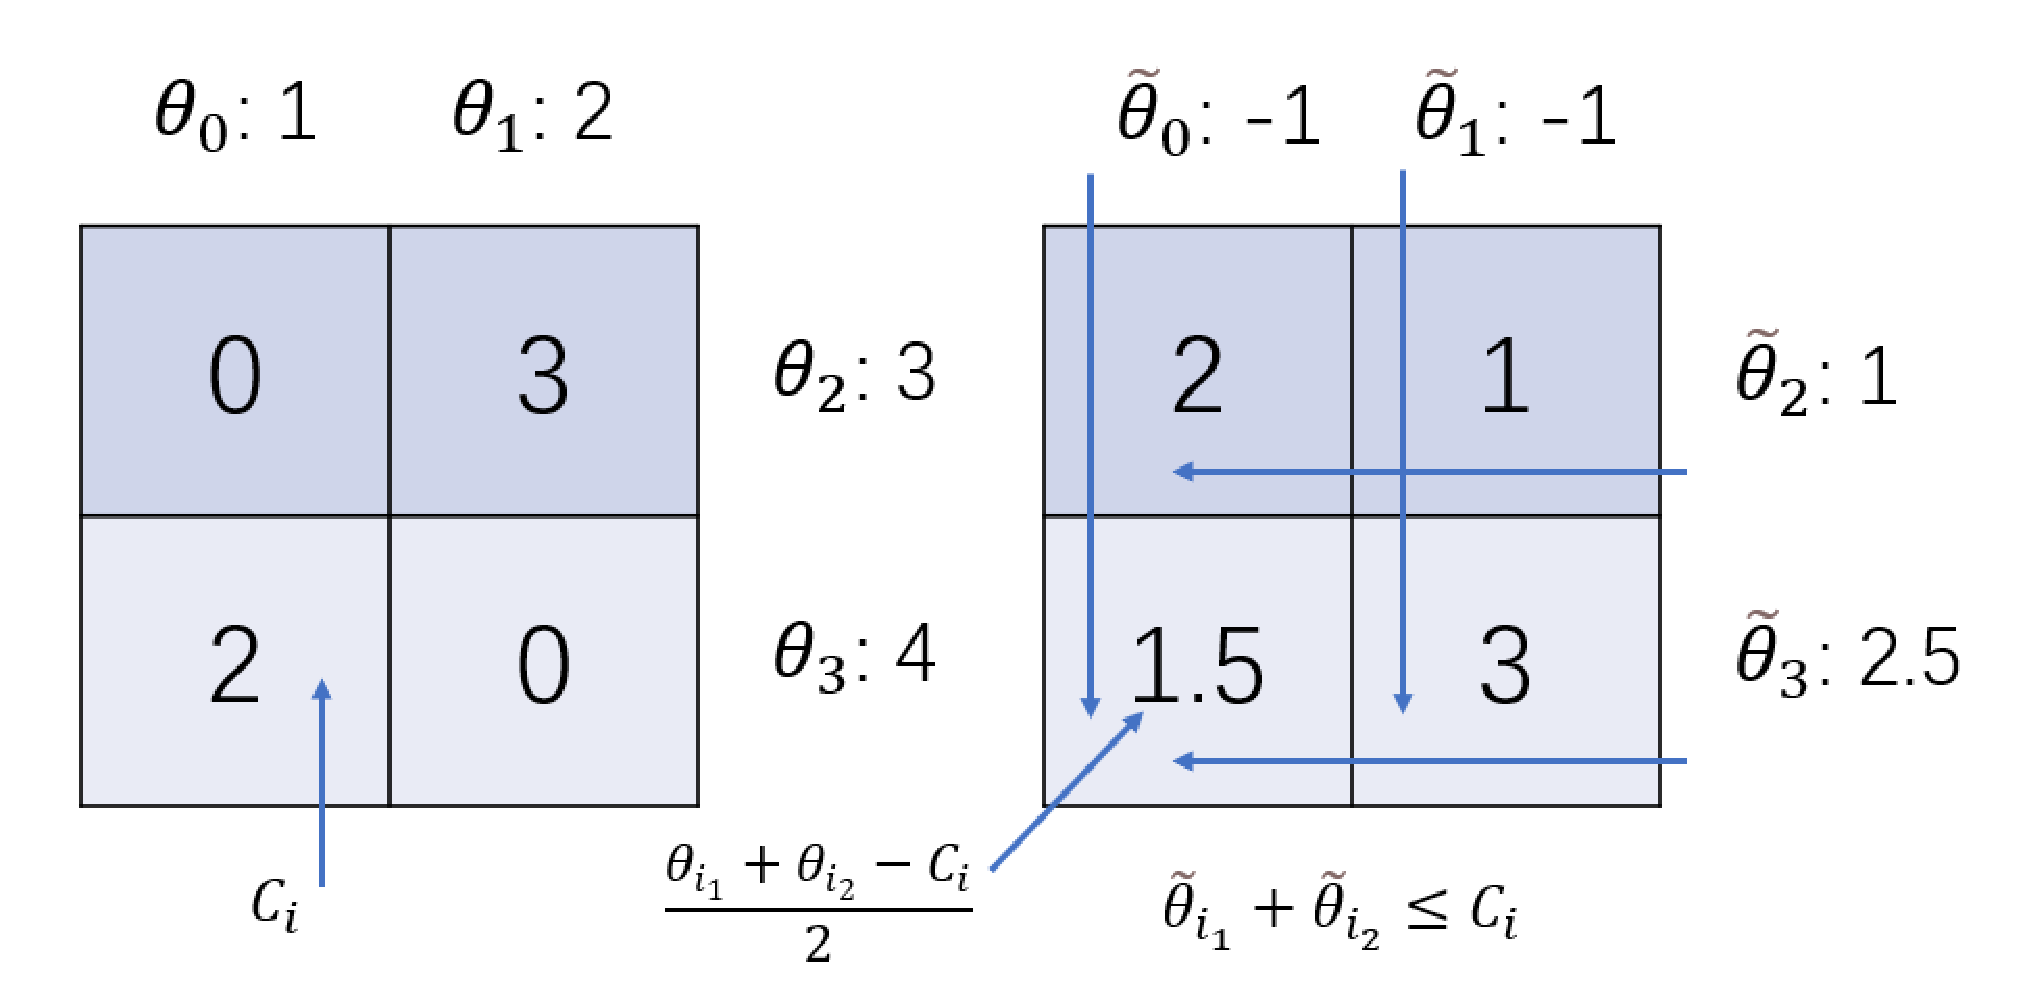
\includegraphics[width = \linewidth]{pic/shifting}
	\caption{Shifting on a 2$\times$2 matrix}
	\end{center}	
	\end{figure}


As we have got the $\tilde{\theta}$ in the $R^{D}$ and we also have another constraint area $\mathcal{R}^{C}$, we are sure that the $\hat{\vt} \in \mathcal{R}^{C}\cap\mathcal{R}^{D}$. However, The intersection of a sphere and a polytope can not be computed in $O(knm)$, where $k$ is a constant. We design a relaxation method. which divides the constraints into two parts, then we maximize the intersection of two hyperplanes and a hyper-ball. 

	\begin{figure}[h]
	\begin{center}	
	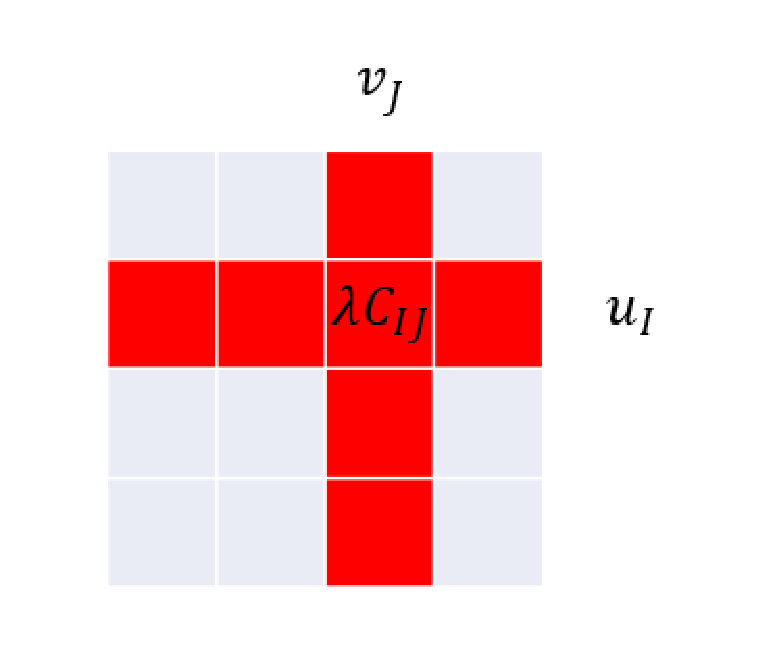
\includegraphics[width = \linewidth]{pic/divide}
	\caption{Selection of group $A_{IJ}$(red) and $B_{IJ}$(grey)}
	\end{center}	
	\end{figure}

\begin{thm}\label{area}(Two plane Screening for UOT) For every single primal variable $t_p$, let $A_p = \{ i \| 0\leq i<nm, i\mid m = I \vee i\mod m = J\}$, $B_p = \{ i \| 0\leq i<nm, i \notin A_p\}$. we can construct the specific area $\mathcal{R}^{S}_{IJ}$ for it.
 \begin{equation}
\begin{split} 
\mathcal{R}^S_{IJ} = \{\theta \|
\begin{aligned}
 &\sum_{l\in A_p}(\theta^{\tranT}\x_{l}\vt_l - \lambda \vc_l \vt)\leq 0 \\
 &\sum_{l\in B_p}(\theta^{\tranT}\x_{l}\vt_l - \lambda \vc_l \vt)\leq 0 \\
  &(\theta-\tilde{\theta})^{\tranT}(\theta-\y)\leq 0
\end{aligned}
\}
\end{split}
\label{eq:divide}
\end{equation}
\end{thm}
We divide the constraints into two groups $A_p$ and $B_p$ for every single $p$, this problem can be solved easily by the Lagrangian method in constant time, the computational process is in Appendix. A


\subsection{Screening Algorithms}

 \begin{algorithm}
 \caption{UOT Dynamic Screening Algorithm}
 \begin{algorithmic}[h]
 \renewcommand{\algorithmicrequire}{\textbf{Input:}}
 \renewcommand{\algorithmicensure}{\textbf{Output:}}
 \REQUIRE $\vt_0, S \in R^{n\times m}, S_{ij}=1, (i,j) = mi+j$
 \ENSURE $S$
 \STATE \text{Choose a solver for the problem.}
 \FOR {$k = 0 \text{ to } K$}
 \STATE $\text{Projection } \tilde{\theta} = \operatorname{Proj}(t^k)$ 
 \FOR {$i = 0 \text{ to } m$}
  \FOR {$j = 0 \text{ to } n$}
  \STATE $\mathcal{R}^{S} \Leftarrow \mathcal{R_{ij}}^S{(\tilde{\theta},t^k)}$
   \STATE $S \Leftarrow {S_{ij} = 0 \text{ if } \max_{\theta \in \mathcal{R}^S} {x_{(i,j)}}^{\tranT}\theta <\lambda c_{(i,j)} }$
 \ENDFOR
  \ENDFOR
 \FOR {$(i,j) \in \{(i,j)\|S_{ij}=0\}$}
  \STATE $\vt^k_{(i,j)} \Leftarrow 0$
  \ENDFOR
  \STATE $\vt^{k+1} = \operatorname{update}(\vt^k)$
 \ENDFOR
  
 \RETURN $\vt^{K+1}, S $ 
 \end{algorithmic} 
 \end{algorithm}

The screening method is irrelevant to the optimization solver you choose. We give the specific algorithm for $L_2$ UOT problem to show the whole optimization process. The $\operatorname{update}$ indicates the updating process for $\vt$ according to the optimizer you choose.\\












































%\section{Experiments}
In this section, we show the efficacy of the proposed methods using a toy Gaussian model and the MNIST dataset.
\subsection{Screening Ratio}
%\section{Conclusion}
Our algorithm is great, we are going to apply the method onto Sinkhorn

\begin{abstract}
\note{HK comment:  We change the story: (OT and UOT $\rightarrow$ Lasso-type UOT $\rightarrow$ Propose Screening (No literature) $\rightarrow$ Evaluation)}
The safe screening technique saves computational time by freezing the zero elements in the sparse solution of the Lasso problem. Recently, researchers have linked the UOT problem to the Lasso problem. In this paper, we propose a dynamic screening method to the $\ell_2$-norm penalized unbalanced optimal transport (UOT) problem. We first apply the screening method to the UOT problem. We find out that the specific structure for the UOT problem allows it to get better screening results than the Lasso problem. We propose the new Dynamic Screening algorithm and demonstrate its extraordinary effectiveness and potential to benefit from the unique structure of the UOT problem, our algorithm substantially improves the screening efficiency compared to the standard Lasso Screening algorithm without significantly increasing the computational burden. We demonstrate the advantages of the algorithm through some experiments on the Gaussian distributions and the MNIST dataset.
\end{abstract}


\section{INTRODUCTION}
\label{sec:int}
Optimal transport (OT) has a long history in mathematics and has recently become \changeXS{popular} in machine learning and statistical learning \changeXS{due to its excellence }in measuring the distance between two probability measures. It has outperformed traditional methods in many different areas such as domain adaptation \citep{Courty_PAMI_2017}, generative models \citep{arjovsky2017wasserstein}, graph machine learning \citep{Maretic_NIPS_2019} and natural language processing \citep{Chen_ICLR_2019}. The popularity of OT is attributed to the introduction of the Sinkhorn's algorithm \citep{Sinkhorn_1974} for the entropy-regularized Kantorovich formulation problem \citep{Cuturi_NIPS_2013}, which alleviates the computational burden in large-scale problem. 

Addressing one limitation that the standard OT problem handles only {\it balanced} samples, the unbalanced optimal transport (UOT) has been proposed envisioning a wider range of applications with {\it unbalanced} samples \citep{Caffarelli_AM_2010,chizat2017scaling}. This application fields include, for example, computational biology \citep{Schiebinger_CELL_2019}, machine learning \citep{Janati_AISTATS_2019} and deep learning \citep{Yang_ICLR_2019}. Mathematically, UOT replaces the equality constraints with penalty functions on the marginal distributions with a divergence including KL divergence \citep{Liero:2018wo}, and $\ell_1$-norm \citep{Caffarelli_AM_2010} and $\ell_2$-norm distances \citep{refId0}. The KL-penalized UOT with an entropy regularizer can be solved by the Sinkhorn algorithm \citep{UOTSinkhorn2020}. It is fast, scalable, and differentiable, but suffers from \changeXS{instability \citep{DBLP:journals/corr/Schmitzer16}, larger error, and a lack of sparsity in solution compared with other regularizers} \citep{Blondel_AISTATS_2018}. In contrast, $\ell_2$-norm regularized UOT not only \changeXS{has} a lower error but also brings a sparse solution. This attracted the attention of researchers to \changeXS{develop new and faster optimization algorithms} \citep{Blondel_AISTATS_2018, Nguyen_arXiv_2022}.

Despite of the success in the development of fast and efficient optimization algorithms for UOT, computational burden still remains as a bottleneck for large-scale applications. This paper tackles this issue from a different direction independent of optimization algorithms. Recently, \cite{Chapel_NeurIPS_2021} suggested a mutual connection between the UOT problem and the Lasso-like problem \citep{Tibshirani_JRSS_1996,Efron_AM_2004} and the non-negative matrix factorization problem \citep{Lee_NIPS_2000}. This motivates us to adapt {\it safe screening} \citep{ghaoui2010safe} in these fields to accelerate the computation of the UOT problem. In fact, the OT and UOT problems expect the solution to be sparse due to the effectiveness of their optimal transport cost, and thus shares the similar idea with the Lasso problem. 
%Hence, we believe that it indicates the potential effectiveness of applying screening techniques in the Lasso problem to the UOT problem. 
Safe screening in the Lasso problem is a promising technique to speed up the computation by exploiting the sparsity of the solution. It eliminates elements in the solution that are guaranteed to be zero without solving the optimization problem. This does not affect the final solution. However, this straightforward application is not trivial, and the standard Lasso screening method cannot be applied directly to the UOT problem because it has un-regularized elements \note{(what means?)}. 
%Fortunately, the UOT problem has a particular structure compared to the Lasso problem. 
Specifically, while the Lasso problem has a dense {\it constraint matrix}, that of the UOT problem is extremely sparse and has a unique transport matrix structure. This would benefit a design of specialized screening method and the outcome. 
%


In this paper, we propose a new dynamic screening method designated to the UOT problem. To this end, we first derive a dual formulation of the vectorized Lasso-like UOT problem. Then, particularly addressing the structure of the constraint matrix, a dynamic screening method is derived, which includes a new projection method and a safe screening region construction method. These are suitable for the UOT problem and could largely improve the effects. Different from the screening method in the Lasso problem, our proposed methods are .......



\textbf{Contributions.}: 
\begin{itemize}
\item To the best of our knowledge, this work is a first dynamic screening method designated to the UOT problem, which is based on the Lasso-like formulation of the UOT problem and its dual formulation. Our proposed method is independent of optimization algorithms.
\item We propose a projection method by leveraging the specific structure of the UOT problem, and it largely decreases the errors in the projection process. 
We also propose a flexible two hyper-plane method  for every primal element to construct the safe screening region.
\item Numerical evaluation reveals their effectiveness in terms of projection distances and screening ratios comparing with several methods including state-of-the-art methods.
\end{itemize}


The paper is organized as follows. {\bf Section \ref{sec:pre}} presents preliminary descriptions of optimal transport and unbalanced optimal transport. The screening methods in Lasso-like problems are explained by addressing a dynamic screening framework. In {\bf Section \ref{sec:pro}}, our proposed screening method for the UOT problem is detailed. {\bf Section \ref{sec:exp}} shows numerical experiments.

\section{PRELIMINARIES}
\label{sec:pre}

$\mathbb{R}^n$ denotes $n$-dimensional Euclidean space, and $\mathbb{R}^n_+$ denotes the set of vectors in which all elements are non-negative. $\mathbb{R}^{m \times n}$ represents the set of $m \times n$ matrices. Also, $\mathbb{R}^{m \times n}_+$ stands for the set of $m \times n$ matrices in which all elements are non-negative. We present vectors as bold lower-case letters $\vec{a},\vec{b},\vec{c},\dots$ and matrices as bold-face upper-case letters $\mat{A},\mat{B},\mat{C},\dots$. The $i$-th element of $\vec{a}$ and the element at the $(i,j)$ position of $\mat{A}$ are represented respectively as $a_i$ and \changeHK{${A}_{i,j}$. The $i$-th column of $\mat{A}$ is represented as $\vec{a}_i$.} In addition, $\one_n \in \mathbb{R}^n$ is the $n$-dimensional vector in which all the elements are one. For $\vec{x}$ and $\vec{y}$ of the same size, $\langle \vec{x},\vec{y} \rangle = \vec{x}^T\vec{y}$ is the Euclidean dot-product between vectors. For two matrices of the same size $\mat{A}$ and $\mat{B}$, $\langle \mat{A},\mat{B}\rangle={\rm tr}(\mat{A}^T\mat{B})$ is the Frobenius dot-product. We use $\|\vec{a}\|_2$ and $\|\vec{a}\|_1$ to represent the $\ell_2$ norm and $\ell_1$ norm of $\vec{a}$, respectively. 
%For a vector $\vec{x}$, the $i$-th element of $\exp (\vec{x})$ and $\log (\vec{x})$ respectively represent $\exp (\vec{x}_i)$ and $\log (\vec{x}_i)$. $\mathrm{KL}(\vec{x},\vec{y})$ stands for the KL divergence between $\vec{x} \in \mathbb{R}_+^n$ and $\vec{y} \in \mathbb{R}_+^n$, which is defined as $\sum_i \vec{x}_i \log {(\vec{x}_i/\vec{y}_i)} - \vec{x}_i + \vec{y}_i$. 
$D_\phi$ is the Bregman divergence with the strictly convex and differentiable function $\phi$, i.e., $D_\phi(\vec{a},\vec{b})=\sum_{i} d_\phi(a_i, b_i)=\sum_i [\phi(a_i) - \phi(b_i) - \phi'(a_i)(a_i -b_i)]$. In addition, we suggests a vectorization for $\mat{A} \in \mathbb{R}^{m \times n}$ as a lowercase letters $\vec{a} \in \mathbb{R}^{mn}$ and $\vec{a}=\text{vec}(\mat{A})=[\mat{A}_{1,1}, \mat{A}_{1,2}, \cdots, \mat{A}_{m,n-1}, \mat{A}_{m,n}]$.
 


\subsection{Optimal Transport and Unbalanced Optimal Transport}
{\bf Optimal Transport (OT):} Given two discrete probability measures $\vec{a}\in \R^{m}$ and $\vec{b} \in \R^{n}$, the standard OT problem seeks a corresponding {\it transport matrix} $\mat{T} \in \R_{+}^{m \times n}$ that minimizes the total transport cost \citep{Kantorovich_1942}. This is a linear programming problem formulated as
\begin{eqnarray}
\label{Eq:Standard_OT}
\operatorname{OT}(\vec{a},\vec{b}) &:=& \min_{ \mat{T} \in \R_{+}^{m \times n}} \langle \mat{C}, \mat{T} \rangle \\
\text{subject\ to}&& \mat{T} \one_n= \vec{a}, \mat{T}^{T}\one_m = \vec{b}, \notag
\end{eqnarray}
where $\mat{C} \in \mathbb{R_{+}}^{m \times n}$ is the {\it cost matrix}. The constraints in (\ref{Eq:Standard_OT}) are so-called {\it mass-conservation constraints} or {\it marginal constraints}, and assume $\|\vec{a}\|_1 = \|\vec{b}\|_1$. Thus, the solution $\hat{\vec{t}}$ does not exist when $\|\vec{a}\|_1 \neq \|\vec{b}\|_1$. The obtained OT matrix $\mat{T}^*$ brings powerful distances as $\mathcal{W}_p = \langle \mat{T}^*,\mat{C} \rangle^{\frac{1}{p}}$, which is known as the $p$-th order {\it Wasserstein distance} \citep{Villani_2008_OTBook}. 


As $\vec{t} = \text{vec}({\mat{T}}) \in \mathbb{R}^{mn}$ and $\vec{c} = \text{vec}({\mat{C}}) \in \mathbb{R}^{mn}$, we reformulate Eq.(\ref{Eq:Standard_OT}) in a vector format as \citep{Chapel_NeurIPS_2021}
\begin{eqnarray}
\label{Eq:Vector_OT}
\operatorname{OT}(\vec{a},\vec{b}) &:=& \min_{\vec{t} \in \R_{+}^{mn}} \vec{c}^T\vec{t} \\
\text{subject\ to}&& \mat{N}\vec{t} = \vec{a}, \mat{M}\vec{t} = \vec{b}, \notag
\end{eqnarray}
where $\mat{N} \in \R^{m \times mn}$ and $\mat{M} \in \R^{n \times mn}$ are two matrices composed of ``0" and ``1". $\mat{N}$ and $\mat{M}$ in case of $m=n=3$ are given, respectively, as
\begin{equation*}
\begin{split}
\mat{N}&=\begin{pmatrix}
1&1&1& 0& 0& 0& 0& 0&0\\
0 & 0& 0&1&1&1& 0& 0&0\\
0 & 0& 0& 0& 0& 0&1&1&1\\
\end{pmatrix},\\
\mat{M}&=\begin{pmatrix}
 1& 0& 0&1& 0& 0&1& 0&0\\
 0&1& 0& 0&1& 0& 0&1&0\\
 0& 0&1& 0& 0&1& 0& 0&1\\
 \end{pmatrix}.
  \end{split}
 \end{equation*}

Note that $\mat{N}$ and $\mat{M}$ both have a specific structure, where each column has only one single non-zero element equal to $1$. 

 
{\bf Unbalanced Optimal Transport (UOT):} The marginal constraints in (\ref{Eq:Standard_OT}) may exacerbate degradation of the performance of some applications where weights need not be strictly preserved. In contrast, the UOT problem {\it relaxes} them by replacing the equality constraints with penalty functions on the marginal distributions with a divergence. Formally, defining $\vec{y} = [\vec{a}, \vec{b}]^T \in \mathbb{R}^{mn}$ and $\mat{X} = [\mat{M}^T,\mat{N}^T]^T \in \mathbb{R}^{(m+n) \times mn}$, the UOT problem can be formulated introducing a penalty function for the histograms as \citep{Chapel_NeurIPS_2021}
\begin{equation}
\label{eq:uot}
\operatorname{UOT}(\vec{a},\vec{b}) := \min_{\vec{t} \in \R_{+}^{mn}} \vec{c}^T\vec{t} + D_\phi(\mat{X}\vec{t},\vec{y}).
\end{equation}

It is worth mentioning that this function is convex due to the convexity of the Bregman divergence.

{\bf Relationship with Lasso-like problem:} 
The Lasso-like problem has a general formula:
%
\begin{eqnarray*}
f(\vec{t}) &:=& g(\vec{t}) + D_\phi(\mat{X} \vec{t},\vec{y}).
%, t\in \mathbb{R}^{mn}.
\end{eqnarray*}
Substituting $g(\vec{t}) = \lambda \|\vec{t}\|_1~(\lambda > 0)$ and $D_\phi(\mat{X} \vec{t},\vec{y}) = \frac{1}{2}\|\mat{X} \vec{t}-\vec{y}\|_2^2$ into $f(\vec{t})$ above reduces to the standard $\ell_2$-norm regularized Lasso problem. On the other hand, addressing that $\vec{c}$ and $\vec{t}$ in (\ref{eq:uot}) are nonnegative, the term $\vec{c}^T\vec{t}$ is represented as $\vec{c}^T\vec{t}=\sum_i c_i t_i = \sum_ic_i |t_i|$. Therefore, the UOT problem in (\ref{eq:uot}) is equivalent to a weighted $\ell_1$-norm regularized Lasso-like problem. It is, however, that $\mat{X} = [\mat{M}^T,\mat{N}^T]^T$ in (\ref{eq:uot}) substantially differs from that of the Lasso problem. More concretely, the former $\mat{X}$ has a specific structure and has only two non-zero elements equal to $1$ in each row whereas the latter $\mat{X}$ in Lasso problem is non-structured and dense \citep{Chapel_NeurIPS_2021}.

\subsection{Dynamic Screening Framework}
Solutions of many large-scale optimization problems tend to be sparse, and a large amount of computation is wasted on updating the zero elements during the optimization process. Screening technique is a well-known technique in the Lasso problem and the SVM problem \citep{Ogawa_ICML_2013}, where the $\ell_1$-norm regularizer leads to a sparse solution for the problem \citep{ghaoui2010safe}. It can pre-select solutions that must be zero theoretically and freeze them before optimization computation, thus saving optimization time. Many safe screening methods have been proposed in this past decade \citep{Liu_ICML_2014,Wang_JMLR_2015}, and recent dynamic screening methods efficiently drop variable elements, which include Dynamic Screening \citep{7128732}, Gap Safe screening \citep{JMLR:v18:16-577} and Dynamic Sasvi \citep{Yamada_NIPS_2021}.

Hereinafter, we briefly elaborate on the framework proposed in \citep{Yamada_NIPS_2021} to introduce the whole dynamic screening technique for the Lasso-like problem:
\begin{equation}
\label{eq:lassolike}
\min_{\vec{t}} \left\{ f(\vec{t}) := g(\vec{t}) + h(\mat{X} \vec{t}) \right\}.
\end{equation}

The Fenchel-Rockafellar Duality yields the dual problem as presented below:
\begin{thm}[Fenchel-Rockafellar Duality {\citep{Rockafellar_Springer_1998}}] 
\label{Thm:FRD}
If $d$ and $g$ are proper convex functions on $\mathbb{R}^{m+n}$ and $\mathbb{R}^{mn}$. Then we have the following:
\begin{equation}
\label{Eq:FRD}
\min_{\vec{t}} g(\vec{t}) + h(\mat{X}\vec{t}) = \max_{\vec{\vec{\theta}}} -h^*(-\vec{\theta})-g^*(\mat{X}^T\vec{\theta}).
\end{equation}
\end{thm}

Because the primal function \changeHK{$h$} is always convex, the dual function \changeHK{$h^*$} is concave. Assuming \changeHK{$h^*$} is an $L$-strongly concave problem, we can design an area for any feasible $\tilde{\vec{\theta}}$ by the strongly concave property:

\begin{thm}[$L$-strongly concave {\citep[Theorem 5]{Yamada_NIPS_2021}}]
\label{thm:circle}
Considering problem in Eq.(\ref{eq:lassolike}), if function $h$ and $g$ are both convex, for $\forall \ \tilde{\vec{\theta}}$ and satisfied the constraints on the dual problem, we have the following area constructed by its L-strongly concave property:  
$$
\begin{aligned}
\mathcal{R}:=\vec{\theta} \in \left\{\frac{L}{2}\|\vec{\theta}-\tilde{\vec{\theta}}\|_2^2+h^*(-\tilde{\vec{\theta}}) \leq h^*(-\vec{\theta})\right\}.
\end{aligned}
$$
\end{thm}

%{\bf Theorem \ref{thm:circle}} yield the following circle constraint. 
\begin{thm}[Circle constraint for Lasso-like problem {\citep[Theorem 8]{Yamada_NIPS_2021}}]
\label{Thm:CC}
Consider the Lasso-like problem and Fenchel-Rockafellar Duality by Eq.(\ref{Eq:FRD}). We assume that $\tilde{\vec{\theta}}$ is inside the domain of dual problem. Then, $\mathcal{R}$ in {\bf Theorem \ref{thm:circle}} is equivalent to the following circle constraint $\mathcal{R}^{C}$:
\begin{equation}
\mathcal{R}^{C} :=\{\vec\theta\ |\ (\vec{\theta}-\tilde{\vec{\theta}})^T(\vec{\theta}-\vec{y})\leq 0\}.
\label{eq:uotcircle}
\end{equation}
$\vec\theta$ and $\vec y$ are the endpoints of the diameter of this circle, and $\hat{ \vec\theta} \in \mathcal{R}^{C}$.
\end{thm}

\note{??We know that the optimal solution $\hat{\vec{\theta}}$ for the dual problem satisfied the inequality, so the set is not empty.??}


\section{PROPOSED UOT SCREENING}
\label{sec:pro}

This section proposes a new safe screening region $\mathcal{R}^S$ for the UOT problem, and a projection method to perform our dynamic screening based on $\mathcal{R}^S$. $\mathcal{R}^S$ is composed of the circle constraint $\mathcal{R}^C$ in {\bf Theorem \ref{Thm:CC}} and the relaxed region of the dual feasible area $\mathcal{R}^D$. After deriving the dual formulation of the Lasso-like formulated UOT problem in Eq.(\ref{eq:uot}) and $\mathcal{R}^D$, we derive $\mathcal{R}^S$ by relaxing $\mathcal{R}^D$. 
%
Concrete proofs of lemma and theorems are provided in the supplementary file.
\subsection{Safe region construction}

{\bf Dual formulation of UOT:} The UOT problem has the form of
$h(\mat{X} \vec{t}) = \frac{1}{2}\|\mat{X} \vec{t}-\vec{y}\|_2^2$ and $g(\vec{\theta})=\lambda \vec{c}^{T}\vec{t}$, where $t_i \geq 0$ for $i \in [mn]$ in Eq.(\ref{eq:lassolike}). Also, $\vec{\theta} = [\vec{\alpha}^T,\vec{\beta}^T]^T \in \mathbb{R}^{m+n}$, where $\vec{\alpha}\in\R^{m}$ and $\vec{\beta}\in\R^{n}$. We obtain the dual form by {\bf Theorem \ref{Thm:FRD}}:
\begin{lem}[Dual form of UOT problem]
For the UOT problem in Eq.(\ref{eq:uot}), we obtain the following dual problem:
\begin{equation}
\begin{split}
-h^*(-\vec{\theta}) - g^*(\mat{X}^T\vec{\theta})& = -\frac{1}{2}\|\vec{\theta}\|_2^2+\vec{y}^T\vec{\theta} \\
\text{subject\ to} \quad \quad \vec{x}_p^T\vec{\theta} -\lambda c_p &\leq 0, \quad \forall p \in [mn],
\end{split}
\label{eq:uotdual}
\end{equation}
where $\vec{x}_p $ corresponds to the $p$-th column of $\mat{X}$.
\end{lem}
The strongly concave coefficient $L$ for the dual function $f$ is 1. 

{\bf Dual feasible region $\mathcal{R}^D$:} 
The constraint in Eq.(\ref{eq:uotdual}) specifies a dual variable feasible area, denoted as $\mathcal{R}^{D}$, and the optimal dual solution $\hat{\vec{\theta}} \in \mathcal{R}^{D}$ because of {\bf Theorem \ref{thm:circle}}.

The KKT condition of the UOT problem holds for the optimal primal and dual solutions $ \hat{\vec{t}}$ and $\hat{\vec{\theta}}$ that:
\begin{thm}[KKT condition] For the primal optimal solution $\hat{\vec{t}}$ and the dual optimal solution $\hat{\vec{\theta}}$, we have the following relationship:
 \begin{equation}
\begin{split}
\vec{x}_p^T\hat{\vec{\theta}} -\lambda c_p \left\{
\begin{aligned}
< 0 \quad& \Longrightarrow \quad\hat{t}_p = 0\\
= 0 \quad& \Longrightarrow \quad\hat{t}_p \geq 0.
\end{aligned}
\right.
 \end{split}
 \label{eq:kkt}
\end{equation}
\end{thm}

Eq.(\ref{eq:kkt}) indicates a potential method to screen the primal variable $\vec{t}$. However, since we do not know the optimal dual solution $\hat{\vec{\theta}}$ directly, this paper seeks a safe screening region for sceening, denoted as $\mathcal{R}^{S}$, as small as possible that contains the $\hat{\vec{t}}$. In other words, if
\begin{equation}
\label{eq:kktineq}
\max_{\vec{\theta} \in \mathcal{R}^S}\quad  \vec{x}_p^T\vec{\theta} -\lambda c_p < 0.
\end{equation}
then we assert 
%\begin{equation}
$\vec{x}_p^T\hat{\vec{\theta}} -\lambda c_p < 0$,
%\end{equation}
which means the corresponding $\hat{{t}}_p = 0$, and can be screened out. 

For this purpose, we focus on the special structure of $\mat{X}$ in the UOT problem, i.e., the $p$-th column of $\mat{X}$ has only two nonzero elements equal to 1. Defining $(u,v)=(p \mid n,v= p \mod n)$, we rewrite $\vec{x}_p^T\hat{\vec{\theta}} -\lambda c_p < 0$ as
%
\begin{equation}
\alpha_{u} + \beta_{v}-\lambda c_p < 0.
\end{equation}

If we obtain $\tilde{\vec{\theta}}$ in $\mathcal{R}^{D}$, combining $\mathcal{R}^{D}$ with $\mathcal{R}^{C}$ in {\bf Theorem \ref{Thm:CC}}, we can use $\mathcal{R}^{C}\cap\mathcal{R}^{D}$ as the area $\mathcal{R}^{S}$ in Eq.(\ref{eq:kktineq}). The problems difficulties are (i) $\mathcal{R}^{D}$ is hard to calculate, and (ii) we need $\tilde{\vec{\theta}}$ is inside $\mathcal{R}^{D}$. We address two issues below:

{\bf Relaxed feasible region $\mathcal{R}^D$ and safe screening region $\mathcal{R}^S$:} 
However, maximizing on the intersection of a hyper-ball and a polytope cannot be computed easily cause the $(n+m)$-polytope has $nm$ Facets, \note{(????)} which costs too much for a screening operation. 

The most direct method for dealing with the problem is to {\it relax} the polytope constraint into a hyper-plane constraint. Thus, considering the specific structure of the $\mat X$ in the UOT problem, our proposed method relaxes the polytope into two planes by combining the $nm$ dual constraints with a positive weight $t_p \geq 0$, If the constraint is relevant to the dual elements $u$ and $v$, which would influence the screening of $t_p$, we add it in the group $A$, and the rest constraints are added in the group $B$. 
%
More concretely, we divide the polytope constraints into two groups $\changeHK{I_p}$ and $\changeXS{{I}^{C}_p}$ for every $p$, Our two-planes area $\mathcal{R}^S_{p}$ is smaller than the relaxation in \citep{Yamada_NIPS_2021}. Benefiting from the structure of $\vec{x}_p$ and $\vec{x}_p^T\vec{\theta} = {\alpha}_{v} + {\beta}_{v}$, these two dual elements are the optimization directions \note{(???)}, and only $m+n$ constraints are directly connected with them. Dividing the constraints in two groups by whether exists $\alpha_{u}$ and ${\beta}_{v}$ can \note{????alleviate the huge relaxation influence of other secondary dual variables???}. 

\begin{thm}[Two-plane safe screening region for UOT]
\label{Thm:AreaScreeningUOT}
For every single primal variable $t_p$, let $\changeHK{I_p} = \{ i \ | \  0\leq i<nm, \changeHK{u = i\mid n \vee v = i\mod n}\}$, and $\changeXS{{I}^{C}_p} = \{ i \ | \  0\leq i<nm, i \notin \changeHK{I_p}\}$. Then, we construct a specific area $\mathcal{R}^{S}_{p}$ as presented below:
\changeXS{
\begin{equation}
\label{Eq:FinalRS}
\begin{split} 
\mathcal{R}^S_{p}(\vec{\theta}, \vec{t}):= \left\{\vec{\theta} \ \left|\ 
\begin{aligned}
 &\sum_{l\in \changeHK{I_p}}(\vec{x}_{l}^{T}\vec{\theta} - \lambda {c}_l)t_l\leq 0, \\
 &\sum_{l\in \changeXS{{I}^{C}_p}}(\vec{x}_{l} ^{T}\vec{\theta}- \lambda {c}_l)t_l\leq 0, \\
  &(\vec{\theta}-\tilde{\vec{\theta}})^T(\vec{\theta}-\vec{y})\leq 0
\end{aligned}
\right.
\right\}.
\end{split}
\end{equation}
}

\end{thm}

Consequently, we have $\hat{\vec{t}} \note{\ (not\ \hat{\vec{\theta}}????)} \in \mathcal{R}^{C}\cap\mathcal{R}^{D} \subset \mathcal{R}^{S}_{p}$ \note{(A simple proof process might be required for the $\subset$ relationship in the supplementary material)}.
We designate this as {\it two-plane screening} in this paper. This problem can be solved easily by the Lagrangian method in constant time. Its computational process is detailed in supplementary material. A.


\note{(Lagrangian function is around here. )}

\subsection{Projection method}

Before we start to screening with the safe screening region $\mathcal{R}^S$ that is constructed by {\bf Theorem \ref{Thm:AreaScreeningUOT}}, we first have to find a dual variable $\tilde{\vec{\theta}}\in\mathcal{R}^{D}$. Although there exists a relationship between the primal variable and dual variable that $\vec{\theta} = \vec{y} - \mat{X}\vec{t}$, inevitably, we often get $\vec{\theta} \notin \mathcal{R}^{D}$. This requires us to project $\vec{\theta}$ onto $\mathcal{R}^{D}$. Our dynamic screening gets a more accurate screening outcome because the optimization algorithm gradually provides $\vec t^{k} \rightarrow \hat{\vec t}$, and also the dual variable $\vec \theta^{k} \rightarrow \hat{\vec \theta}$. If $\vec{ \tilde{\theta}}\rightarrow \hat{\vec \theta}$, the safe screening region $\mathcal{R}^{C}\cap\mathcal{R}^{D}$ would get smaller and has a better screening outcome. As $\mathcal{R}^{D}$ is a polytope combined with $nm$ hyperplanes, the real projection is solved no matter by Linear programming or Dykstra's projection algorithm. However, its cost is nontrivial. To this issue, in the Standard Lasso problem, the dual constraints in {Eq.(\ref{eq:uotdual})} is $\|\vec{x}_p \hat{\vec{\theta}}\|_1\leq \lambda$, where $\vec{x}_p$ is almost dense and non-structured, one uses a simple shrinking method to obtain a $\tilde{\vec{\theta}} \in \mathcal{R}^{D}$ as 
$
%\begin{equation*}
\tilde{\vec{\theta}} = \frac{\vec\theta}{\max(1, \|{\mat{X}^T\vec\theta}/{\lambda}\|_{\infty})}
%\end{equation*}
$ {\citep[Theorem 11]{Yamada_NIPS_2021}}. 
One straightforward extension of this into the UOT problem could be  
\begin{equation*}
\tilde{\vec{\theta}} = \frac{\vec\theta}{\max(1, \|\frac{\mat{X}^T\vec\theta}{\lambda \vec{c}^{T}}\|_{\infty})}, 
\end{equation*}
where $(\frac{\ \cdot\ }{\cdot})$ is the element-wise division. However, this projection pushes $\vec{\theta}$ far away from the optimal solution $\hat{\vec{\theta}}$ because it suffers from the influence of a small $c_p$. Also, it will degenerate when one of the costs is $c_p = 0$, and disables the screening process. 
%
Therefore, noting that the UOT problem, only allows $t_p \geq 0$, and the $\vec{x}_p$ only consists of two non-zero elements, we can adapt a better and cheap projection method. Specifically, we shift every single $\alpha_u$, $\beta_v$ with half of the maximum differences in all of its constraints.
%

The following theorem states this:
\begin{thm}[UOT shifting projection]
\label{Thm:UOT_ShiftProjection}
For any $\vec{\theta} = [{\vec{\alpha}}^T,{\vec{\beta}}^T]^T$, we define the projection operator $\tilde{\vec{\theta}}={\rm Projection}(\vec{\theta})$, where 
\changeXS{
\begin{eqnarray}
\tilde{{\alpha}}_u &=& {{\alpha}}_u - \max_{0\leq j < n} \frac{{{\alpha}}_u +{{\beta}}_j - \lambda{c}_{un+j}}{2} \notag\\
\tilde{{\beta}}_v &=& {{\beta}}_v - \max_{0 \leq i < m} \frac{{{\alpha}}_i +{{\beta}}_v - \lambda{c}_{in+v}}{2}\\
\label{eq:uotproj}
\end{eqnarray}
}
Then, the calculated $\tilde{\vec{\theta}} = [\tilde{\vec{\alpha}}^T,\tilde{\vec{\beta}}^T]^T$ is inside $\mathcal{R}^{D}$.
\end{thm}
The proof is in the supplementary material. Note that this cheap projection method can get good accuracy with $O(knm)$ computational time. 

\begin{figure}[h]
\begin{center}
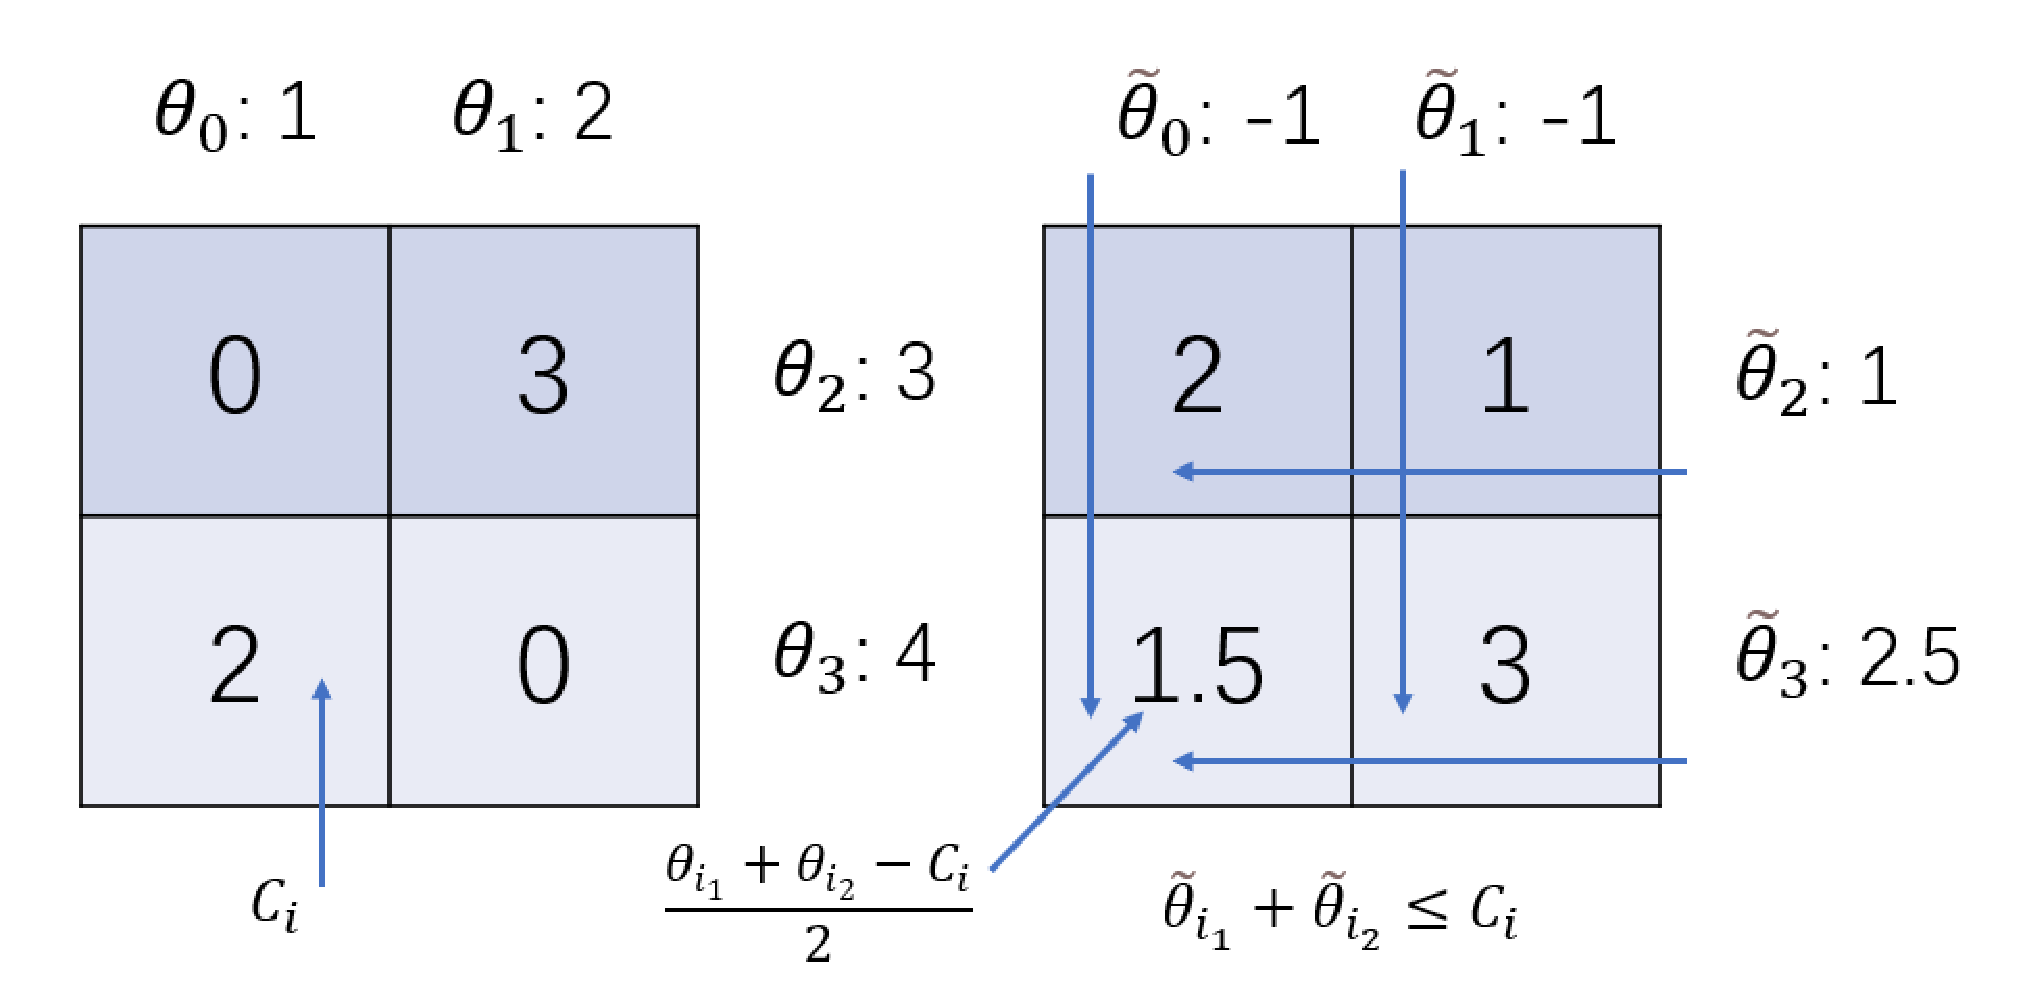
\includegraphics[width = \linewidth]{pic/shifting}
\caption{Shifting on a 2$\times$2 matrix. \note{(To be modified)}}
\end{center}
\end{figure}



\begin{figure}[h]
\begin{center}
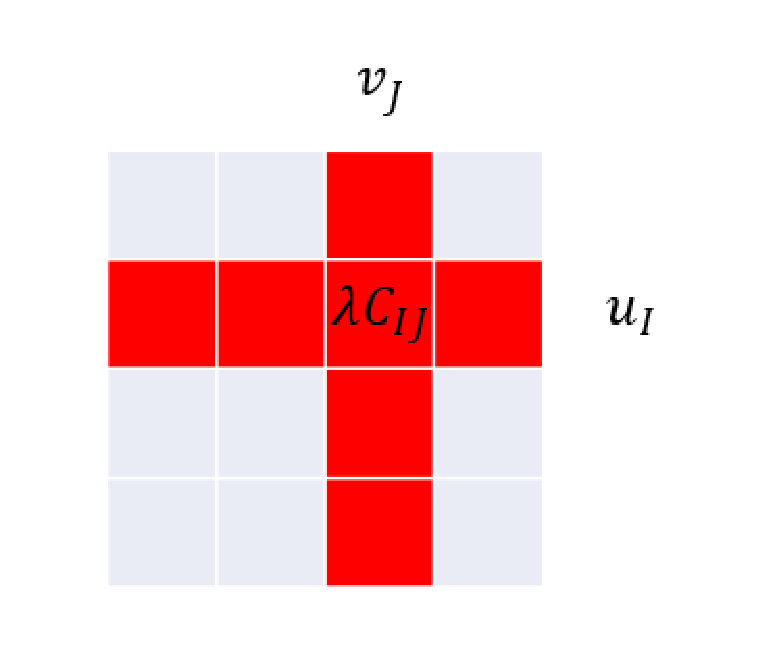
\includegraphics[width = 0.7\linewidth]{pic/divide}
\caption{Selection of group $A_{IJ}$(red) and $B_{IJ}$(grey)}
\end{center}
\end{figure}




\subsection{Screening Algorithms}

% \begin{algorithm}
% \caption{UOT Dynamic Screening Algorithm}
% \begin{algorithmic}[h]
% \label{Alg:UOTDynamicScreening}
% \renewcommand{\algorithmicrequire}{\textbf{Input:}}
% \renewcommand{\algorithmicensure}{\textbf{Output:}}
% \REQUIRE $\vec{t}_0,  \changeXS{\vec s \in \mathbb{R}^{nm}, s_{p}=1, \forall p \in [mn]}, r$
% \ENSURE $s$
% \STATE \text{Choose a solver for the problem.}
% \FOR {$k = 0 \text{ to } K-1$}
% \STATE $\tilde{\vec{\theta}^{k}} = \operatorname{Projection}(\vec{\theta}^k)$ \hfill Eq.(\ref{eq:uotproj})
% \FOR {$p = 0 \text{ to } mn -1$}
%  \STATE  \changeXS{$\mathcal{R}^{S} \leftarrow \mathcal{R}_{p}^S{(\tilde{\vec{\theta}^{k}},\vec{t}^k)}$}
%   \STATE{$\vec s \leftarrow {s_{p} = 0 \text{ if} {\displaystyle \max_{\vec{\theta} \in \mathcal{R}^S} {\vec x_{p}}^T\vec{\theta}^{k} <\lambda c_{p} }}$ \hfill Eq.(\ref{Eq:FinalRS})}
%   %\bf Theorem \ref{Thm:AreaScreeningUOT}
%  \ENDFOR
% \FOR  { \changeXS{$p \in \{p\|s_{p}=0\}$}}
%  \STATE ${t}^k_p \leftarrow 0$
%  
%  \ENDFOR
%  \STATE $\vec{t}^{k+1} = \operatorname{update}(\vec{t}^k)$ \hfill \text{(Optimization process)}
% \ENDFOR
%   \RETURN $\vec{t}^{K}, \vec s $
% \end{algorithmic} 
% \end{algorithm}
% 
 \begin{algorithm}
 \caption{UOT Optimization with Dynamic Screening}
 \begin{algorithmic}[h]
 \label{Alg:UOTDynamicScreening}
 \renewcommand{\algorithmicrequire}{\textbf{Input:}}
 \renewcommand{\algorithmicensure}{\textbf{Output:}}
 \REQUIRE $\vec{t}_0,  \vec s \in \mathbb{R}^{nm}, s_{p}=1\ \forall p \in [mn], r$
 \ENSURE $\vec t^{K}$
 %\STATE \text{Choose a solver for the problem.}
 \FOR {$k = 0 \text{ to } K-1$}
 \IF{$k\mod r =0$}
 \STATE $\tilde{\vec{\theta}^{k}} = \operatorname{Projection}(\vec{\theta}^k)$ \hfill Eq.(\ref{eq:uotproj})
 \FOR {$p = 0 \text{ to } mn -1$}
 \STATE $\mathcal{R}^{S} \leftarrow \mathcal{R}_{p}^S{(\tilde{\vec{\theta}^{k}},\vec{t}^k)}$ \hfill Eq.(\ref{Eq:FinalRS})
   \STATE{$\vec s \leftarrow {s_{p} = 0 \text{ if} {\displaystyle \max_{\vec{\theta} \in \mathcal{R}^S} {\vec x_{p}}^T\vec{\theta}^{k} <\lambda c_{p} }}$ \hfill Eq.(\ref{eq:kktineq})}
 \ENDFOR
  \FOR { $p \in \{p \ |\ s_{p}=0\}$}
 \STATE $\text{Freeze\ }{t}^k_p $
 \ENDFOR
  \ENDIF
  \STATE $\vec{t}^{k+1} = \operatorname{update}(\vec{t}^k)$ \hfill \text{(Optimization process)}
 \ENDFOR
  \RETURN $\vec{t}^{K} $
 \end{algorithmic}
 \end{algorithm}

The purpose of screening methods is to remove variable elements that are ignored at the optimization process in the adopted optimization algorithm. For this, we denote $\vec{s} \in \mathbb{R}^{mn}$ as the {\it screening mask vector} for the transport vector $\vec{t}$. Thus, $s_p = 0$ implies that the corresponding $t_p$ should be screened out. We summarize a specific algorithm for $\ell_2$-norm penalized UOT problem to show the entire optimization process as in {\bf Algorithm \ref{Alg:UOTDynamicScreening}}. The $\operatorname{update}(\vec{t})$ operator in the algorithm indicates the updating process for $\vec{t}$ by using an adopted optimizer. $r \in \mathbb{N}$ specifies the period of the screening because the change in screening ratio is not huge if we screen every time. The period $f$ is decided by a user, and the faster converging the optimizer is, the smaller period $r$ is. It should be emphasized that the proposed screening method is {\it independent} of the adopted optimization algorithm. 

\subsection{Computational Cost Analysis}
\changeXS{Our proposed method needs to construct different plans for every single primal element $p$, however, thanks to the special structure of the $\mat X$, For every single $t_p$, the data required for maximizing (by Lagrange method in supplementary material) can be summarized as some specific sum, which can be computed together and reuse for other elements have the same $t \mod m $ or $t \mid m$. It helps us to preserve the whole optimization complexity to $O(kmn)$, $k$ is a constant.}

\section{EXPERIMENTS}
\label{sec:exp}
In this section, \changeXS{we organize some experiments on randomly generated gaussian distributions and MNIST dataset. We proved the projection effectiveness of our method by measuring the distance between the dual variable and the projected point. We compared our proposed Two-plane Dynamic Screening with some state-of-the-art methods. We also applied our Screening method on some famous $l_2$ norm UOT problem solvers like FISTA, BFGS, Lasso (celer), Multiplicative update, and Regularization path to test its speed-up ratio.}
\subsection{Projection Method}
To prove the effectiveness of our projection method compared with the traditional projection method in the Lasso problem, we compared the projection distance and screening ratio with randomly generated Gaussian measures by two projection methods. We set the $\lambda = \frac{\|\mathbf{X}^Ty\|}{100}$ and test for 10 different pairs. We choose the FISTA for solving the $L_2$ penalized UOT problems. \changeXS{Because the standard Lasso projection method would degenerate when $c_p=0$, we add a small constant $\epsilon=0.01$ on the cost matrix for both methods.} Our projection method has only moved the dual point a little to ensure it is inside the $\mathcal{R}^{D}$ the order of magnitude is ignorable. It ensures the projection step would not harm the approximation process for the computational dual solution $\vec\theta^{k}$ to the optimum $\vec \hat {\theta}$.
\begin{figure}[h]
\begin{center}
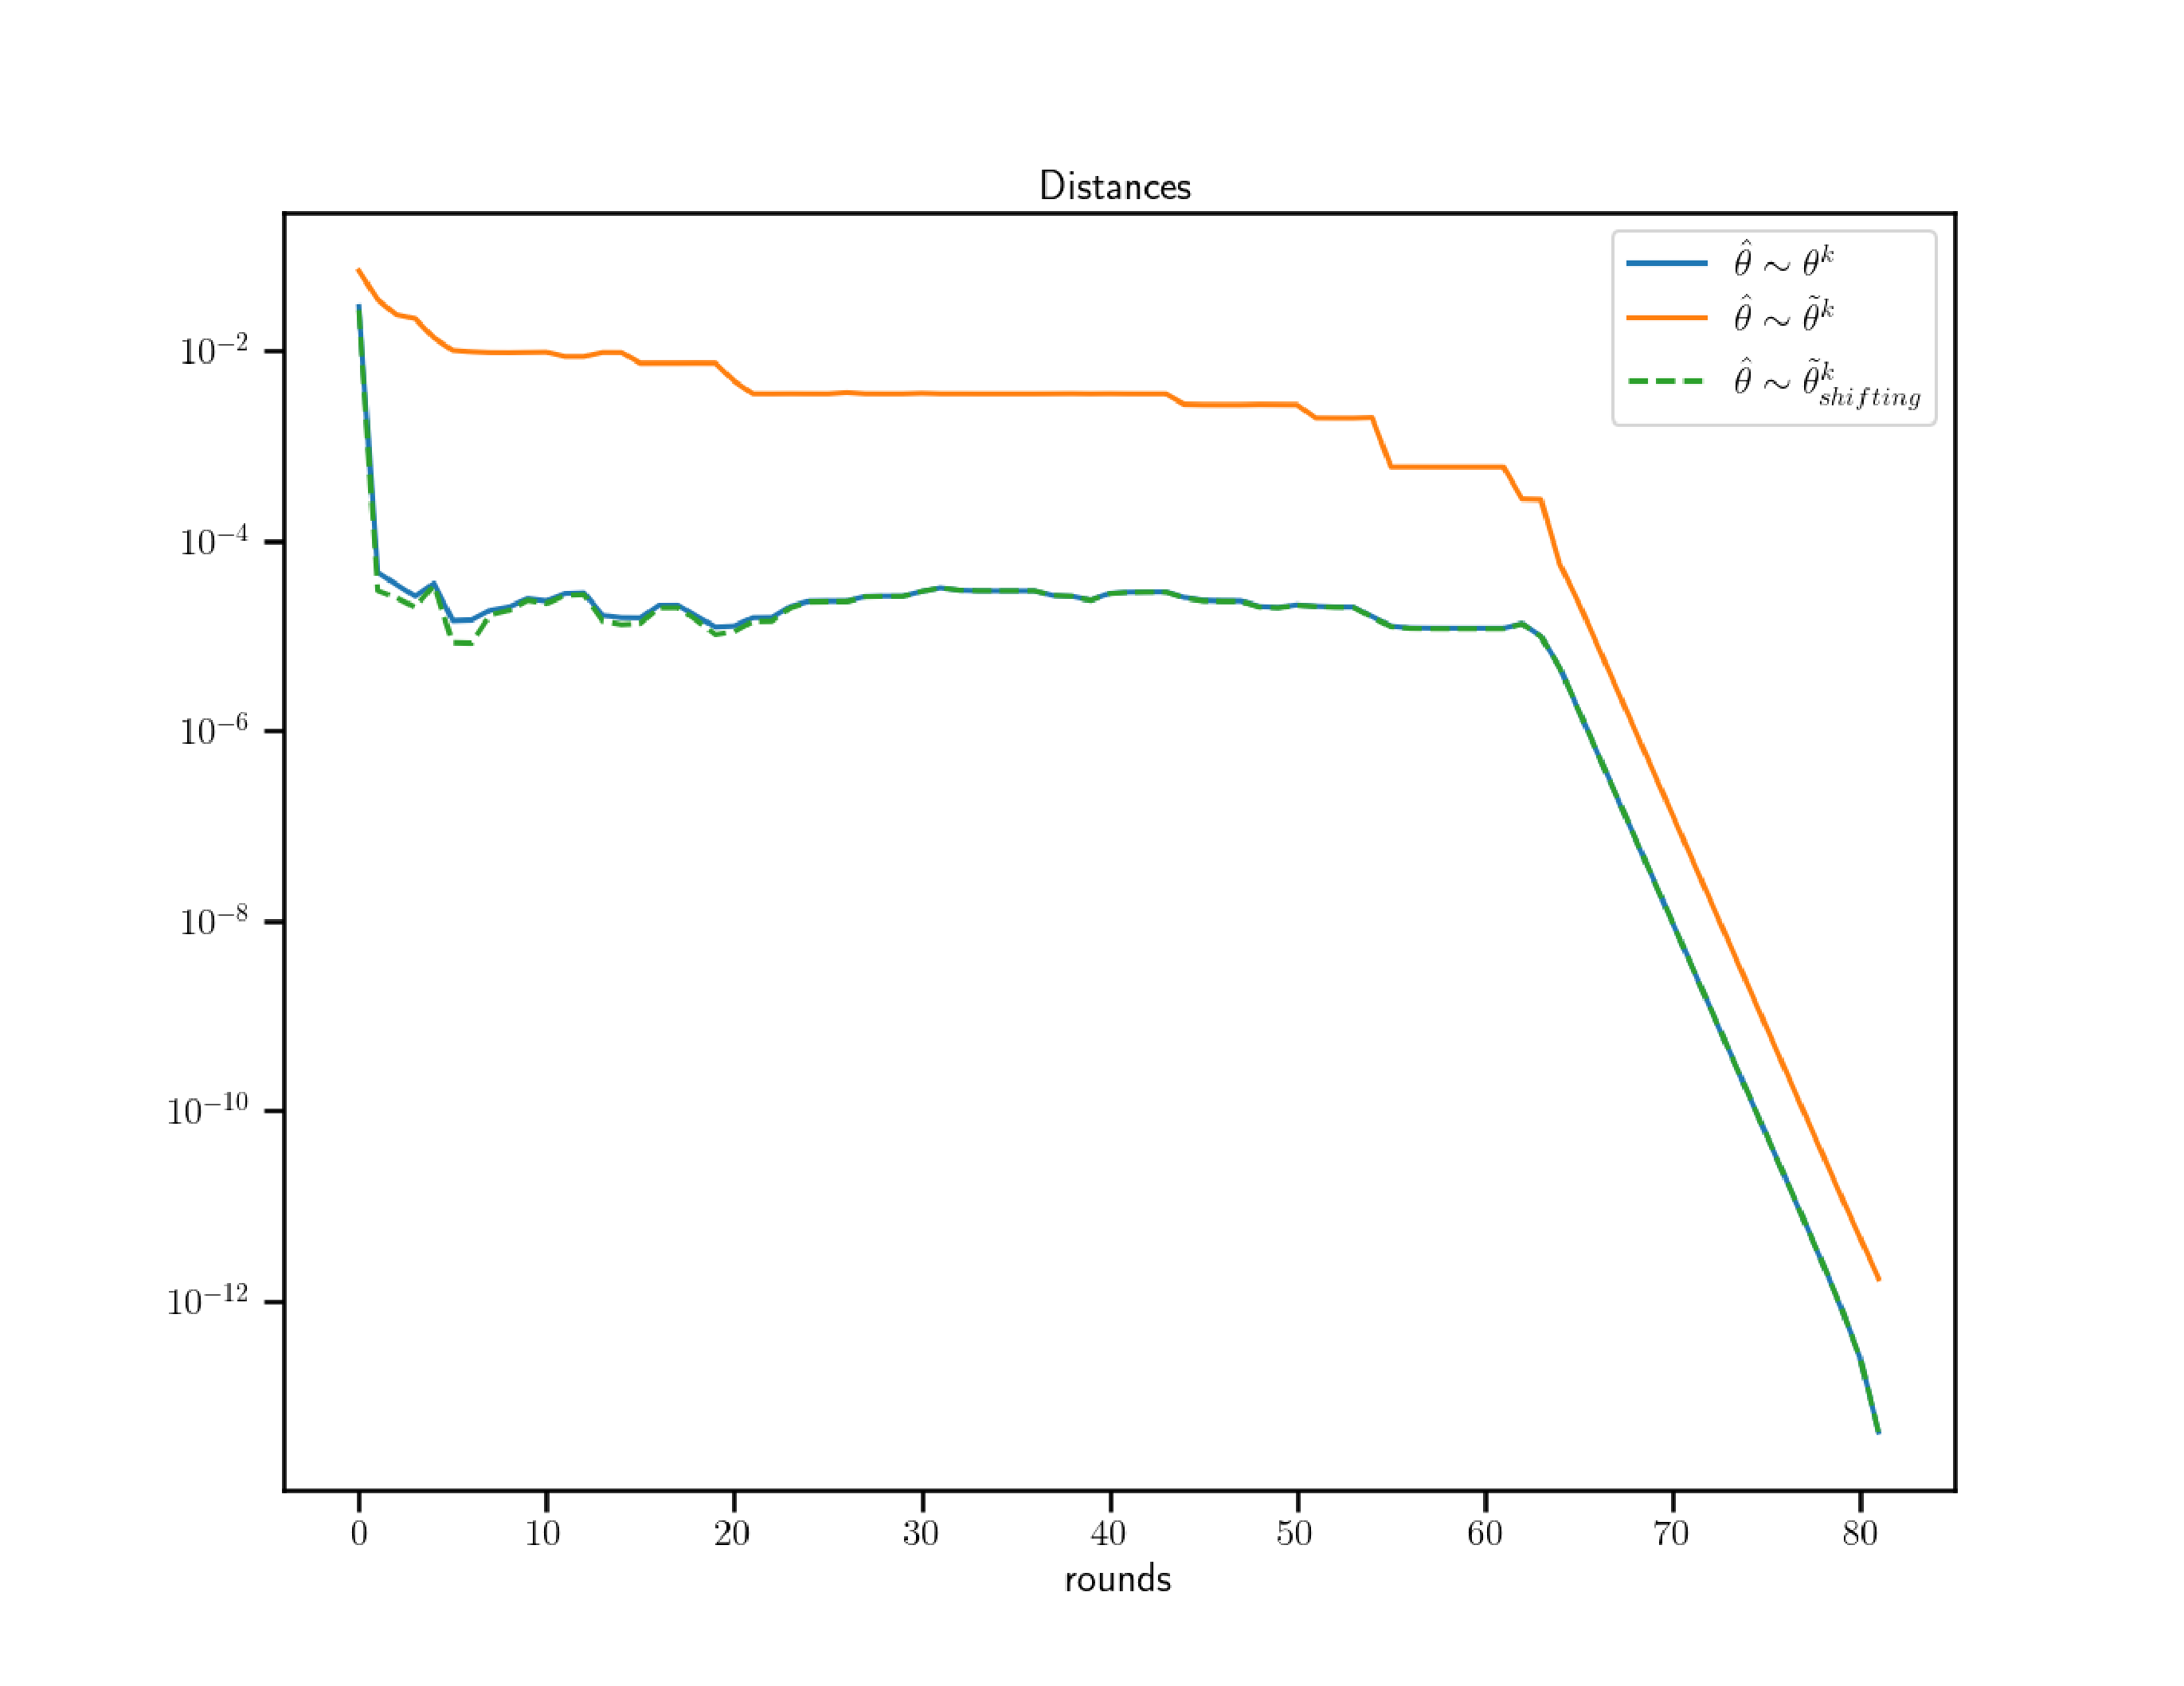
\includegraphics[width = \linewidth]{pic/projdis}
\caption{Distance of different projection method}
\end{center}
\end{figure}
\begin{figure}[htbp]
\begin{center}
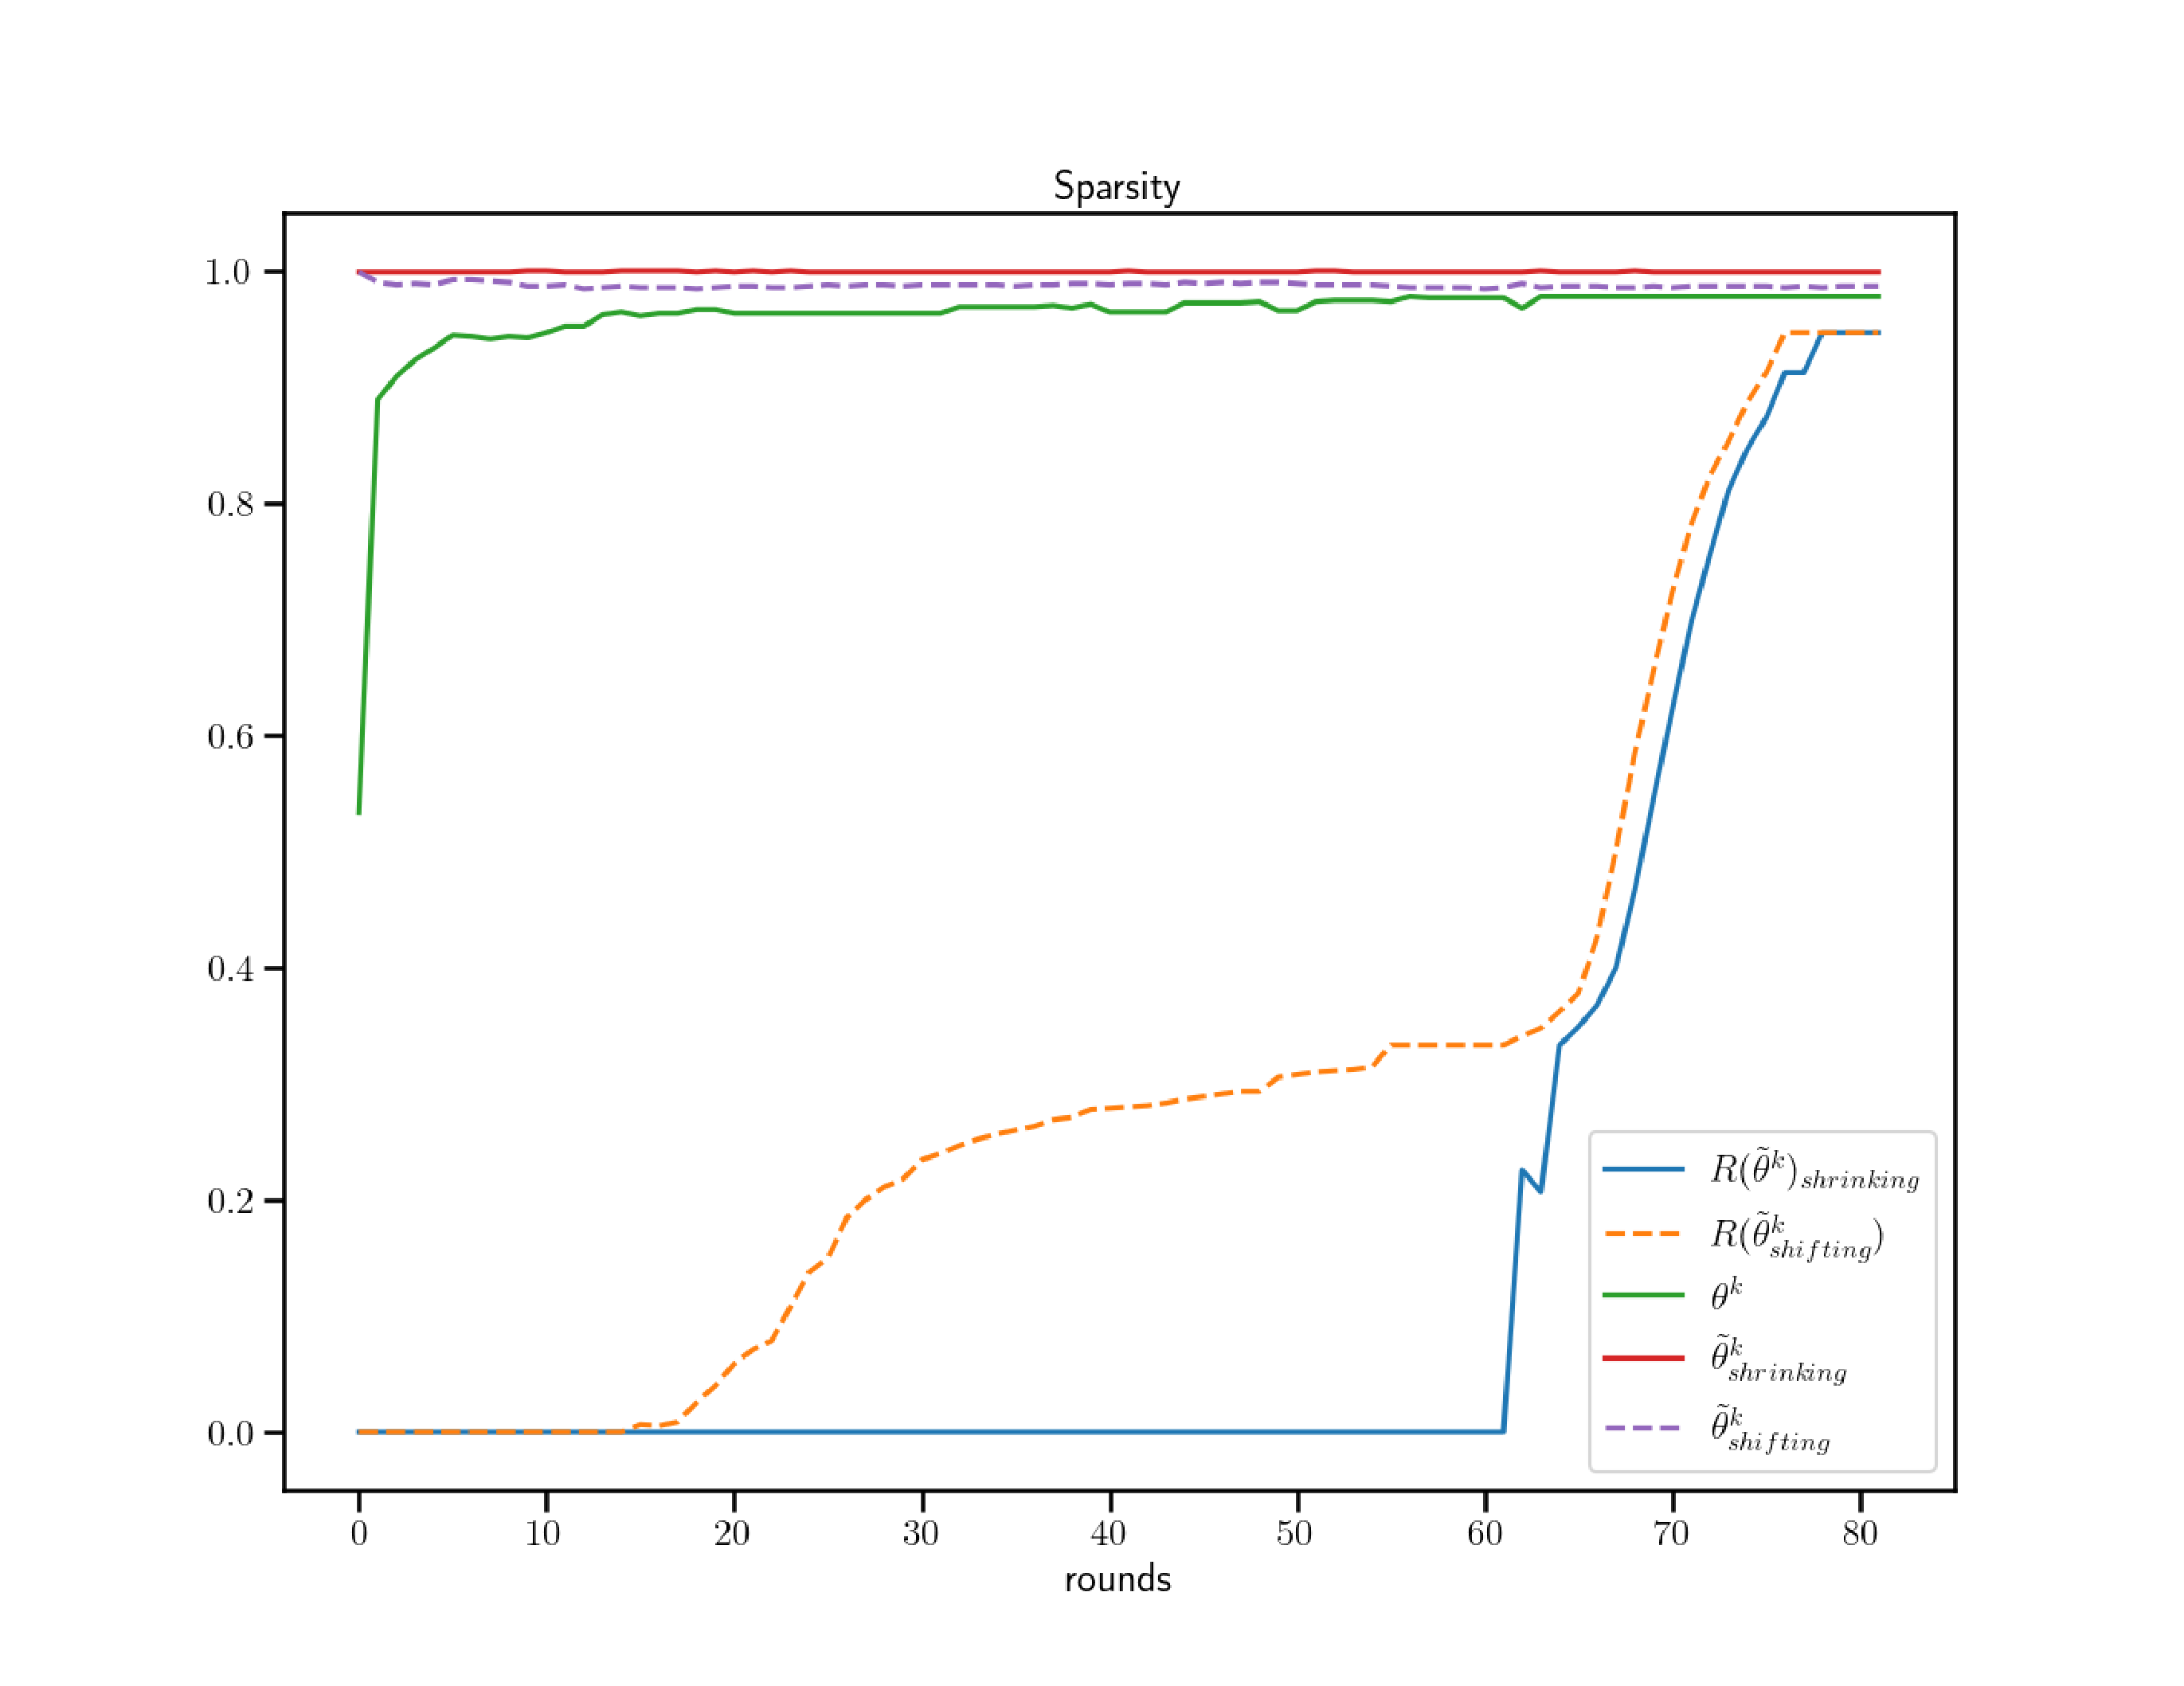
\includegraphics[width = \linewidth]{pic/sparse_proj}
\caption{Screening ratio of different projection method}
\end{center}
\end{figure}

\subsection{Comparing with Other Screening Methods}
We compared the proposed screening ratio with three different methods, \changeXS{including our Cross Two-Plane method (CTP), a Random Two-Plane method (RTP)}, Dynamic Sasvi method, and Gap method. \changeXS{All the methods would use our projection method as it has been proven better than the standard Lasso projection method. It is clear that the CTP still outperform all the other method, CTP can start screening at a very early stage. The RTP just randomly divides the constraints and combines them into two planes, Although RTP is still better than the Sasvi algorithm, the performance is worse than CTP. which indicates that our achievements should not be simply attributed to the choice of more planes, The effectiveness is highly connected with the specific structure of the UOT problem, which decrease the influence of other variables and make us able to divide the constraints according to the variables.}
\begin{figure}[h]
\begin{center}
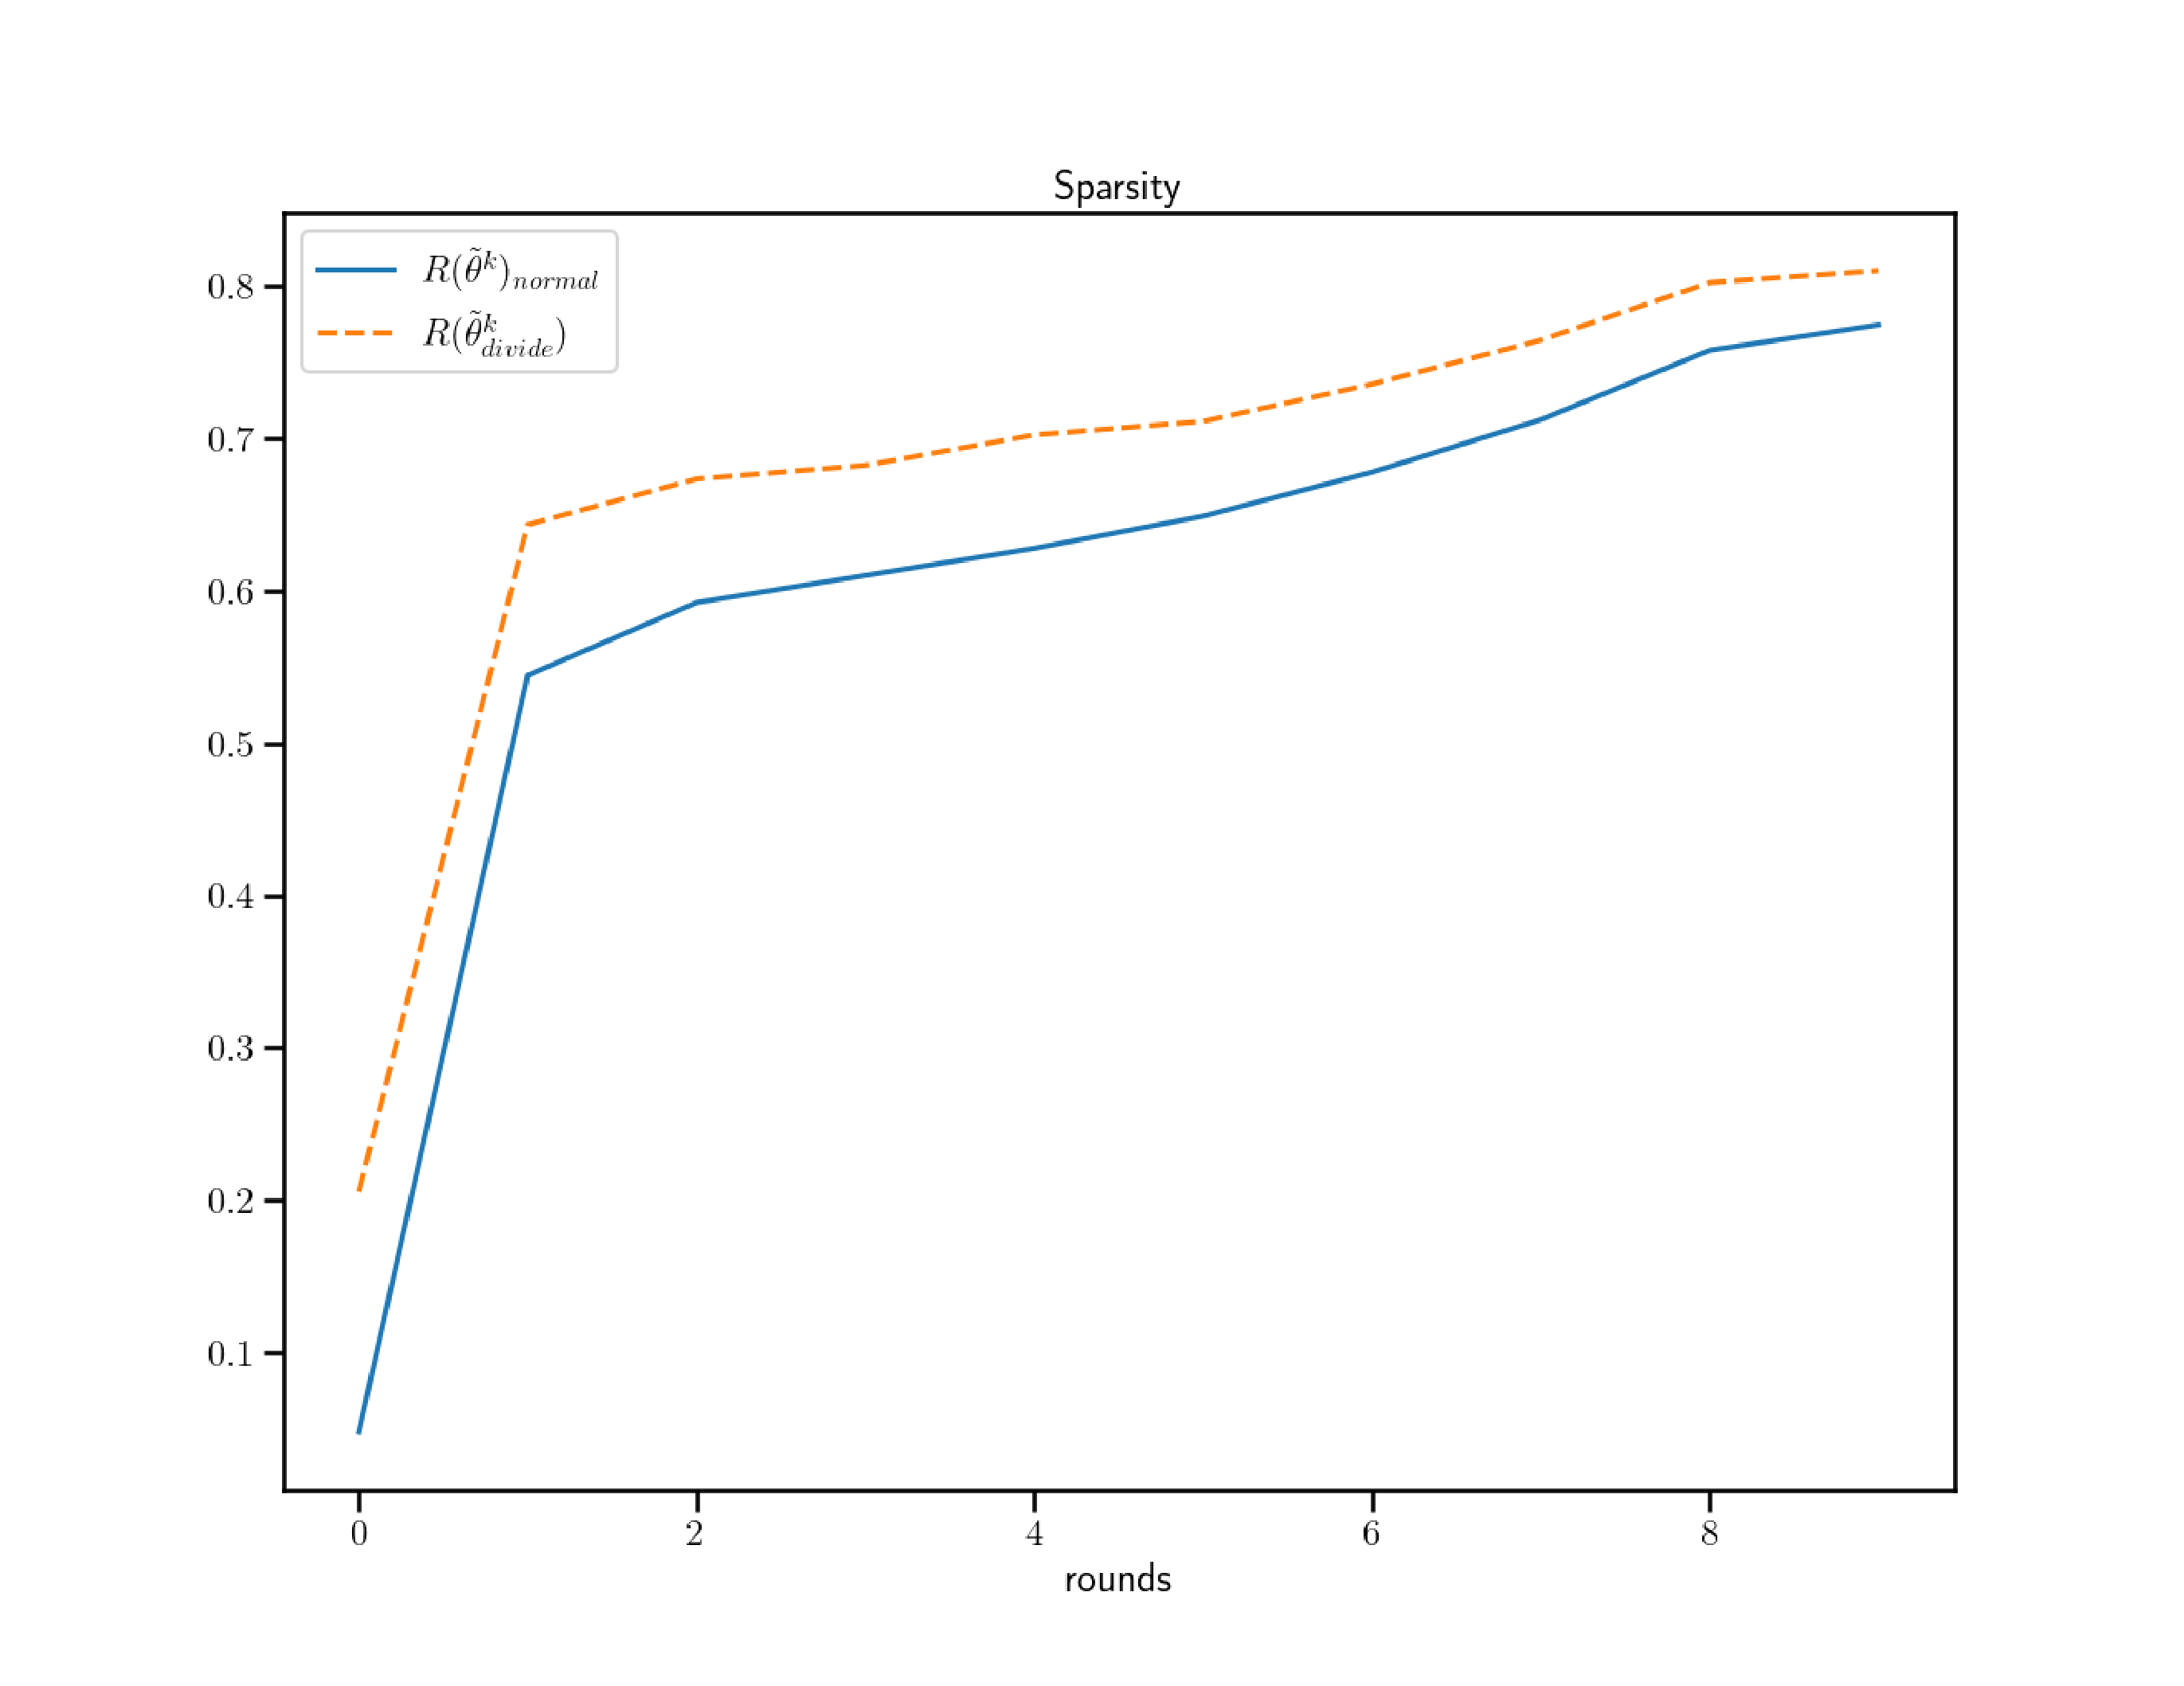
\includegraphics[width = \linewidth]{pic/screening_divide_ratio_long}
\caption{Screening ratio of dividing method}
\end{center}
\end{figure}


\subsection{Speed up Ratio}

\changeXS{We applied the CTP in different UOT optimizers like FISTA, BFGS, Lasso(celer), Multiplicative update, and Regularization path method, and use them to solve the UOT problem between random number figure pairs in the MNIST dataset, we compared the consuming time for different accuracy and showed in the table, Our Screening method can get a good speed up ratio for almost every optimizer, and performs especially good on Multiplicative update algorithms}
	\begin{figure}[h]
	\begin{center}	
	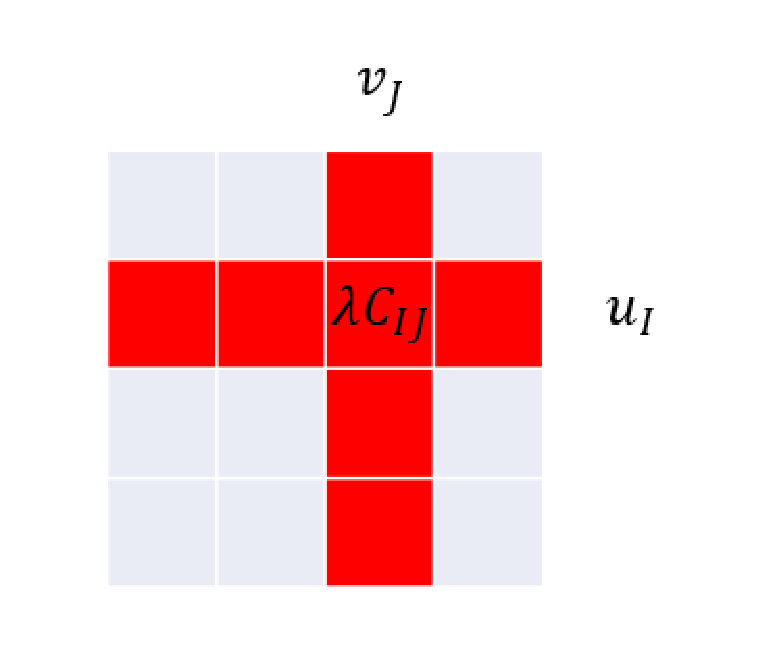
\includegraphics[width = \linewidth]{pic/divide}
	\caption{speed up ratio for different solver}
	\end{center}	
	\end{figure}



\section{CONCLUSION}
\changeXS{This paper introduced the Screening method in the Lasso community to the UOT problem and demonstrates that the screening method has extra potential to make a difference in the UOT community due to its specific structure. We provide a better projection method for the UOT screening process and design a Cross Two-Plane safe Screening region for it, which accomplishes a good performance and shows the potential to exploit the structure of the UOT problem. We believe these approaches can be extended to other regularized and penalized UOT problems like KL penalized UOT \citep{Dantas_ICASSP_2021} problem and even entropic UOT problem. we are going to combine our method with the Sinkhorn algorithm to alleviate its drawbacks on computational time and sparsity.}

\clearpage
\bibliographystyle{apalike}
\bibliography{ref}


%%%%%%%%%%%%%%%%%%%%%%%%%%%%%%%%%%%
%%%%%% SUPPLEMENT (OPTIONAL) %%%%%%
%%%%%%%%%%%%%%%%%%%%%%%%%%%%%%%%%%%

\clearpage
\appendix

\thispagestyle{empty}


% For one-column format, uncomment the following:
\onecolumn \makesupplementtitle
% For two-column format, uncomment the following:
%\twocolumn[ \makesupplementtitle ]

\section{PROOFS}
\subsection{Proof of Theorem \ref{Thm:UOT_ShiftProjection}}
For any $p \in {0,1,...,nm -1}$ we assume that $p = (I,J)$, then we can compute that:
 \begin{equation}
\begin{split} 
\vec{x}_p^T\tilde{\vec{\theta}} &= \tilde{\vec{\alpha}}_{I} + \tilde{\vec{\beta}}_v \\
				    &= {\vec{\alpha}}_{I} + {\vec{\beta}}_v - \max_{0\geq j\geq n} \frac{{\vec{\alpha}}_u +{\vec{\beta}}_j - \lambda \vec{c}_{p}}{2} - \max_{0 \geq i \geq m} \frac{{\vec{\alpha}}_i +{\vec{\beta}}_v - \lambda \vec{c}_{p}}{2}\\
				    &= \frac{{\vec{\alpha}}_{I} + {\vec{\beta}}_J}{2} - \max_{0\geq j\geq n} \frac{{\vec{\beta}}_j}{2} - \max_{0 \geq i \geq m} \frac{{\vec{\alpha}}_i }{2} + \lambda \vec{c}_{p}\\
				    &= \frac{1}{2}\vec{x}_p^T{\vec{\theta}} - \max_{0\geq j\geq n} \frac{{\vec{\beta}}_j}{2} - \max_{0 \geq i \geq m} \frac{{\vec{\alpha}}_i }{2} +\lambda \vec{c}_{p} \\
				    &\leq \lambda \vec{c}_{p} 
 \end{split} 
\end{equation}
For $\forall p$, we have $\tilde{\vec{\theta}} \in \mathcal{R}^{D}$

\subsection{Proof of Theorem \ref{Thm:AreaScreeningUOT}}
We Generalize the problem as 
\begin{equation}
\max_{\vec{\theta} \in \mathcal{R}^{S}_{I}}{ \vec{\theta}_{I_1} +\vec{\theta}_{I_2} }
\end{equation}
Considering the center of the circle as $\vec{\theta}^o$, we define $\vec{\theta} = \vec{\theta}^{o} + q$, as ${ \vec{\theta}^{o}_{I_1} +\vec{\theta}^{o}_{I_2} }$ is a constant, the problem is equal to $\min_{\vec{\theta} \in \mathcal{R}^{S}_{I}}{- ( \vec{q}_{I_1} +\vec{q}_{I_2} )}$, we compute the Lagrangrian function of later:
\begin{equation}
\min_{\vec{q}} \max_{\eta,\mu,\nu \geq 0} L(\vec{q},\eta,\mu,\nu) =\min_{\vec{q}}\max_{\eta,\mu,\nu\geq0} - {\vec{q}_{I_1} - \vec{q}_{I_2} + \eta( \vec{q}^T\vec{q} - r^2)+\mu( a^T\vec{q} - e_a ) + \nu( b^T\vec{q} - e_b )}
\end{equation}

 \begin{equation}
\begin{split} 
\frac{\partial L}{\partial \vec{q}_i} = \left\{
\begin{aligned}
-1 + 2\eta \vec{q}_i +\mu a_i + \nu b_i \quad& i = I_1, I_2\\
 2\eta \vec{q}_i +\mu a_i + \nu b_i \quad& i \neq I_1, I_2
\end{aligned}
\right.
 \end{split}
\label{eq:lang1}
\end{equation}

 \begin{equation}
\begin{split} 
{\vec{q}_i}^{*} = \left\{
\begin{aligned}
\frac{1- \mu a_i - \nu b_i}{2\eta} \quad& i = I_1, I_2\\
-\frac{\mu a_i + \nu b_i}{2\eta} \quad& i \neq I_1, I_2
\end{aligned}
\right.
 \end{split}
\label{eq:lang1}
\end{equation}

We can get the Lagrangian dual problem:
\begin{equation}
\max_{\eta,\mu,\nu\geq0} L(\eta,\mu,\nu) = \max_{\eta,\mu,\nu\geq0} \frac{\mu a_{I_1} + \nu b_{I_1}-1}{2\eta} +\frac{\mu a_{I_2} + \nu b_{I_2}-1}{2\eta}+ \eta({\vec{q}^{*}}^T\vec{q}^{*}-r^2 )+\mu( a^T\vec{q}^{*} - e_a ) + \nu( b^T\vec{q}^{*} - e_b )
\end{equation}
From the KKT optimum condition, we know that if
\begin{equation}
\begin{split} 
 \eta ({\vec{q}^{*}}^T\vec{q}^{*} -r^2) &= 0\\
 \mu( a^T\vec{q}^{*} - e_a)&= 0\\
 \nu(b^T\vec{q}^{*} - e_b) &=0
 \end{split}
\end{equation}
We set $\eta^{*}, \mu^{*}, \nu^{*}$ as the solution of the equations, which is also the solution of the dual problem. Firstly, we assume that $\eta^{*}, \mu^{*}, \nu^{*} \neq 0$, then the solution is equal to compute the following equations:

\begin{equation}
\begin{split} 
 & (1-\mu a_{I_1}-\nu b_{I_1})^2 + (1-\mu a_{I_2}-\nu b_{I_2})^2 + \sum^{m+n}_{i\neq I_1,I_2}(a_i\mu+b_i\nu)^2 - 4\eta^2 r^2 = 0 \\
 & a_{I_1}-\mu a_{I_1}^2-\nu b_{I_1}a_{I_1} + a_{I_2}-\mu a_{I_2}^2-\nu b_{I_2}a_{I_2} - \sum^{m}_{i\neq I_1,I_2}(a_i^2\mu +b_i a_i\nu) - 2\eta {e_a} = 0 \\
 & b_{I_1}-\nu b_{I_1}^2-\mu b_{I_1}a_{I_1} + b_{I_2}-\nu b_{I_2}^2-\mu b_{I_2}a_{I_2} - \sum^{m}_{i\neq I_1,I_2}(b_i^2\nu +b_i a_i\mu) - 2\eta {e_b} = 0 
 \end{split}
\end{equation}
Rearranged as:
\begin{equation}
\begin{split} 
 & 2-2\mu (a_{I_1}+a_{I_2})-2\nu(b_{I_1}+b_{I_2})+ \|a\|^2\mu^2+\|b\|^2\nu^2+2\mu\nu a^Tb - 4\eta^2 r^2 = 0 \\
 & (a_{I_1}+ a_{I_1}) - \|a\|^2\mu - a^Tb\nu - 2\eta {e_a} = 0 \\
 & (b_{I_1}+ b_{I_2}) - \|b\|^2\nu - a^Tb \mu - 2\eta {e_b} = 0 
 \end{split}
\end{equation}

we have 
\begin{equation}
\begin{split} 
\mu &= \frac{2( e_ba^Tb - e_a\|b\|^2 )\eta + (a_{I_1}+a_{I_2}) \|b\|^2 - (b_{I_1} + b_{I_2}) (a^Tb)}{ \|a\|^2 \|b\|^2 -a^Tb}\\
\nu &=\frac{2( e_aa^Tb - e_b\|a\|^2 )\eta + (b_{I_1}+b_{I_2}) \|a\|^2 - (a_{I_1} + a_{I_2}) (a^Tb)}{ \|a\|^2 \|b\|^2 -a^Tb}\\
 \end{split}
\end{equation}
set it as:
\begin{equation}
\begin{split} 
\mu &= s_1 \eta + s_2\\ 
\nu &= u_1 \eta + u_2
 \end{split}
 \label{eq:final}
\end{equation}

Then we can solve the $\eta$ as a quadratic equation:
\begin{equation}
\begin{split} 
0&=a\eta^2+b\eta+c\\
 a&= 4r^2 - s_1^2\|a\|^2 - u_1^2\|b\|^2 -2s_1 u_1a^Tb\\
b&=2(a_{I_1} + a_{I_2})s_1 +2(b_{I_1} + b_{I_2})u_1 - 2s_1s_2 \|a\|^2 - 2u_1u_2\|b\|^2 - 2(s_1u_2+s_2u_1)a^Tb \\
 c&=2(a_{I_1} + a_{I_2})s_2 +2(b_{I_1} + b_{I_2})u_2 -s_2^2\|a\|_1 -u_2^2\|b\|_1 - 2s_2u_2a^Tb -2
 \end{split}
\end{equation}

Then we can put it back into \ref{eq:final} and get $\mu, \nu$.

If the solution satisfied the constraints $\eta^{*}, \mu^{*}, \nu^{*} > 0$, then it is the solution.
However, if one of the dual variables is less than 0, the problem would degenerate into a simpler question. 

If only $\eta^{*}$ is larger than 0, 
 $\min_{\vec{\theta} \in \mathcal{R}^{S}_{I}}{- ( \vec{q}_{I_1} +\vec{q}_{I_2} )} = -\sqrt{2}r$

If only $\mu^{*}$ or $\nu^{*}$ is less than 0, we are optimizing on a sphere cap, the solution can be found in \cite[supplementary material B]{Yamada_NIPS_2021}

if only $\eta^{*} \leq 0$:
As the sphere is inactivated, the problem gets maximum at every point of the intersection of two planes.
\begin{equation}
\min_{\vec{q}} \max_{\mu,\nu \geq 0} L(\vec{q},\mu,\nu) =\min_{\vec{q}}\max_{\mu,\nu\geq0} - {\vec{q}_{I_1} - \vec{q}_{I_2} +\mu( a^T\vec{q} - e_a ) + \nu( b^T\vec{q} - e_b )}
\end{equation}
To have a solution, the equations satisfied
 \begin{equation}
\begin{split} 
\frac{\partial L}{\partial q} = \left\{
\begin{aligned}
-1+\mu a_i + \nu b_i =0 \quad& i = I_1, I_2\\
-\mu a_i -\nu b_i \quad =0& i \neq I_1, I_2
\end{aligned}
\right.
 \end{split}
\end{equation}

As the equation satisfied, we can just set $\vec{q}_i^{*} = 0, i \neq I_1,I_2$, then we compute the  
 \begin{equation}
 \min_{\vec{\theta} \in \mathcal{R}^{S}_{I}}{- ( \vec{q}_{I_1} +\vec{q}_{I_2} )} = \frac{a_{I_2}e_b - b_{I_2}e_a -a_{I_1}e_b +b_{I_1}e_a}{a_{I_1}b_{I_2}-a_{I_2}b_{I_1}}
\end{equation}


\end{document}



